%%%%%%%%%%%%%%%%%%%%%%%%%%%%%%%%%%%%%%%%%%%%%%%%%%%%%%%%%%%%%%%%%%%%%%%%%%%%%%%%%%%%%%%%%%%
%%
%% LaTeX Template for Faculty of ICT at University of Malta
%%
%% The updated version of this document should be downloaded from
%%      https://github.com/jp-um/university_of_malta_LaTeX_dissertation_template
%%
%% In case of any difficulties please contact Dr JP Ebejer on jean.p.ebejer@um.edu.mt
%%
%%%%%%%%%%%%%%%%%%%%%%%%%%%%%%%%%%%%%%%%%%%%%%%%%%%%%%%%%%%%%%%%%%%%%%%%%%%%%%%%%%%%%%%%%%%

%% Before you embark on this quest you should probably read some of:
%% Deadly sins - http://mirrors.ctan.org/info/l2tabu/english/l2tabuen.pdf
%% Writing a thesis in LaTeX - http://tug.org/pracjourn/2008-1/mori/mori.pdf

\RequirePackage[l2tabu, orthodox]{nag} % tells you of any bad LaTeX usage
                                       % must be first thing in class (with the exception of comments)

%% There is one option you should define; oneside or twoside
%% Use twoside for your viva docs (examiners hate long docs they need to carry around)
%% and oneside for the final thing you submit to the library.  Note that margins will
%% change accordingly

\documentclass[oneside]{um-fict}  % custom University of Malta project/dissertation/thesis 


%% **************** (Your) Packages (Start) ******************

% \listfiles % uncomment this to know which packages you are using
              % the list of packages will be in the bottom of the .log file

%% Note that packges may already be loaded from the um (and memoir) classes.
%% Do not add your packages to the template, but rather add them here.

\usepackage{blindtext} %% for some dummy text, remove in your writeup
\usepackage{coffee4}    %% for some fun

%% ***************** (Your) Packages (End) *******************


%% **************** (Your) Data (Start) ******************

\title{Machine Learning Approaches to the Blockchain}  % use \\ here otherwise you get a justified title
                                     % note capitalization of the title (only common 
                                     % words in lower case)
\tagline{some hyped-up tagline}      % tag line
\author{Jean-Paul Ebejer}            % your full name
\authorID{123456M}                   % your University Identifier
\supervisor{Dr Zhivago}              % your supervisor(s) name - no . in Dr
\cosupervisor{Dr Who}                % your cosupervisor(s) name - no . in Dr *OPTIONAL* 
                                     % simply comment out the above line if absent

\degreeName{Some Degree}       		 % the degree you are reading
                                     % note the \ after the dot, so not to consider it a fullstop
\doctype{dissertation}               % the type of document (fyp, dissertation, thesis)
\degreeDate{\monthyeardate\today}    % when did you submit (officially after your corrections)
%%\subjectcode{ICS5200}              % the study unit-code (currently not used)

%% ***************** (Your) Data (End) *******************


%% ******** (Your) Document Settings (Start) *************

% You should have an images directory in every chapX subdir
% NOTE:  Trailing / for subdirs is required.
\graphicspath{{./images/}{./chap1/images/}{./chap2/images/}}   % Paths where to look for images, if defined "images" must always be there as it holds the images in-use by the template.

\makeindex

%% ********* (Your) Document Settings (End) **************

% DOCTOR'S (JP) ORDERS: MAKE SURE TO READ MY TWO BLOG ENTRIES WITH
% CONTENT AND LaTeX TIPS FOR YOUR WRITE-UP.  THESE ARE BASED ON  
% EXAMINER'S FEEDBACK
%
% URLS:
% https://bitsilla.com/blog/2019/03/content-tips-for-your-dissertation-or-project-write-up/
% https://bitsilla.com/blog/2019/01/latex-tips-for-your-dissertation-or-project-write-up/

% end the preamble and start the document

\begin{document}
\frontmatter 
    \maketitle
%%    \begin{copyrightenv}
\end{copyrightenv}
       
%%    \begin{dedication}
{\large{To The Avengers}}\\[5mm]
You know, for saving the world.
\end{dedication}

        % include a dedication.tex file
    \begin{acknowledgements}

Thank you to my supervisor Dr Merlinde Kay for guiding me through my project and keeping me on task. 

Thank you to the UNSW IT support team, for answering my enquiries regarding use of the Katana computational cluster.

Thank you to the ECMWF specialist support team, for answering my enquiries regarding the ERA5 dataset.

Thank you to the NOAA-PSL data team, for answering my enquiries regarding their climate indices.

Thank you to the presenters who ran the American Meteorological Society's Python for Climate and Meteorology 2021 Short Course, including those from the Data Carpentry and MetPy teams, who provided me the basic understanding of relevant Python libraries to complete this thesis project. 

Thank you to various online resources by Project Pythia, the Pangeo community, and the development team for the xarray Python package (especially tutorials by staff from the National Center for Atmospheric Research), whose examples I drew from in creating the code for this project. 

Thank you to the Australian Bureau of Meteorology, for providing access to the BARRA reanalysis dataset, and the NSW Department of Planning and Environment, for providing access to urban density datasets, even though a change in project scope meant these datasets were not used.

Thank you to Dr Jean-Paul Ebejer from The University of Malta, who created this \LaTeX thesis template and made it available for general use.

And in general, thank you to all the people who contributed to the literature, as well as software, which made this research possible.

This research includes computations using the computational cluster Katana supported by Research Technology Services at UNSW Sydney.
\end{acknowledgements}   % include an acknowledgements.tex file
    %% For tips on how to write a great abstract, have a look at
%%	-	https://www.cdc.gov/stdconference/2018/How-to-Write-an-Abstract_v4.pdf (presentation, start here)
%%	-	https://users.ece.cmu.edu/~koopman/essays/abstract.html
%%	-	https://search.proquest.com/docview/1417403858
%%  - 	https://www.sciencedirect.com/science/article/pii/S037837821830402X

\begin{abstract}
This is the abstract. \blindtext
\end{abstract}\if@openright\cleardoublepage\else\clearpage\fi
    \tableofcontents*\if@openright\cleardoublepage\else\clearpage\fi
    \listoffigures\if@openright\cleardoublepage\else\clearpage\fi
    \listoftables\if@openright\cleardoublepage\else\clearpage\fi
    %% will only print what is used ... useful.
%% also acronyms are clickable, which is awesome

\chapter{List of Abbreviations} %% \chapter*{List of Abbreviations} not to appear in LoC
\markboth{List of Abbreviations}{List of Abbreviations}
               
\begin{acronym}\itemsep-20pt\parsep-20pt %% if you remove these spacing params this list becomes huge!

\acro{AAO}{Antarctic Oscillation}
\acro{AAOI}{Antarctic Oscillation Index}
\acro{ABL}{Atmospheric Boundary Layer}
\acro{AMO}{Atlantic Multidecadal Oscillation}
\acro{AMOI}{Atlantic Multidecadal Oscillation Index}
\acro{AO}{Arctic Oscillation}
\acro{AOI}{Arctic Oscillation Index}
\acro{AVHRR}{Advanced Very High Resolution Radiometer}
\acro{AVIM}{Atmosphere-Vegetation Interaction Model}
\acro{AWS}{Automatic Weather Station}
\acro{BLH}{Boundary Layer Height}
\acro{BOM}{(Australian) Bureau of Meteorology}
\acro{C10}{Weibull Scale Parameter for 10 m Wind Speed}
\acro{C100}{Weibull Scale Parameter for 100 m Wind Speed}
\acro{CA}{Central America}
\acro{CAPE}{Convective Available Potential Energy}
\acro{CBH}{Cloud Base Height}
\acro{CCN}{Cloud Condensation Nuclei}
\acro{CDR}{Climate Data Record}
\acro{CFD}{Computational Fluid Dynamics}
\acro{CIAD}{Condensation-Induced Atmospheric Dynamics}
\acro{CPC}{Climate Prediction Center}
\acro{dBLH}{Hourly Change in Boundary Layer Height}
\acro{dCAPE}{Hourly Change in Convective Available Potential Energy}
\acro{dCBH}{Hourly Change in Cloud Base Height}
\acro{dFA}{Hourly Change in Forecast Albedo}
\acro{DJF}{December-January-February}
\acro{DMI}{Dipole Mode Index}
\acro{dMSLP}{Hourly Change in Mean Sea Level Pressure}
\acro{DMWS}{Daily Maximum Wind Speed}
\acro{dNAC}{Hourly Change in Net Atmospheric Condensation}
\acro{dNSE}{Hourly Change in Net Surface Evaporation}
\acro{dSLHF}{Hourly Change in Surface Latent Heat Flux}
\acro{dSSHF}{Hourly Change in Surface Sensible Heat Flux}
\acro{dT2}{Hourly Change in Temperature at 2 m Above Surface}
\acro{dTCC}{Hourly Change in Total Cloud Cover}
\acro{dTCCLW}{Hourly Change in Total Column Cloud Liquid Water}
\acro{dTCWV}{Hourly Change in Total Column Water Vapour}
\acro{dU10}{Hourly Change in Zonal Component of 10 m Wind Velocity}
\acro{dU100}{Hourly Change in Zonal Component of 100 m Wind Velocity}
\acro{dV10}{Hourly Change in Meridional Component of 10 m Wind Velocity}
\acro{dV100}{Hourly Change in Meridional Component of 100 m Wind Velocity}
\acro{dVIDMF}{Hourly Change in Vertical Integral of Divergence of Moisture Flux}
\acro{dVIEC}{Hourly Change in Vertical Integral of Energy Conversion}
\acro{dVIKE}{Hourly Change in Vertical Integral of Kinetic Energy}
\acro{dVIPILE}{Hourly Change in Vertical Integral of Potential, Internal and Latent Energy}
\acro{dWS10}{Hourly Change in Wind Speed at 10 m Above Surface}
\acro{dWS100}{Hourly Change in Wind Speed at 100 m Above Surface}
\acro{dWV10}{Hourly Change in Wind Velocity at 10 m Above Surface}
\acro{dWV100}{Hourly Change in Wind Velocity at 100 m Above Surface}
\acro{ECMWF}{European Centre for Medium-Range Weather Forecasts}
\acro{ENSO}{El Nino-Southern Oscillation}
\acro{EPO}{Eastern Pacific Oscillation}
\acro{EPOI}{Eastern Pacific Oscillation Index}
\acro{ERA5}{ECMWF Reanalysis v5}
\acro{EROE100}{Expected Rate of 100 m Wind Speed Exceeding 42.5 m/s}
\acro{FA}{Forecast Albedo}
\acro{FAPAR}{Fraction of Photosynthetically Absorbed Radiation}
\acro{FWM}{Friction Wind Model}
\acro{GCM}{General Circulation Model}
\acro{GE}{General Electric}
\acro{GLASS}{Global Land Surface Satellite}
\acro{GPP}{Gross Primary Production}
\acro{GW}{Goldwind}
\acro{HPC}{High-Performance Computing}
\acro{IFS}{Integrated Forecasting System}
\acro{IOD}{Indian Ocean Dipole}
\acro{JJA}{June-July-August}
\acro{JMA}{Japanese Meteorological Agency}
\acro{JRA55}{Japanese 55-year Reanalysis}
\acro{K10}{Weibull Shape Parameter for 10 m Wind Speed}
\acro{K100}{Weibull Shape Parameter for 100 m Wind Speed}
\acro{LAI}{Leaf Area Index}
\acro{LCC}{Land Cover Change}
\acro{LCL}{Lifted Condensation Level}
\acro{LOAC}{Large-scale Ocean-Atmosphere Circulation}
\acro{LSE}{Land Surface Elevation}
\acro{LT}{Local Time}
\acro{LULCC}{Land Use and Land Cover Change}
\acro{MAM}{March-April-May}
\acro{MDP}{Mean Diurnal Profile}
\acro{MERRA2}{Modern-Era Retrospective analysis for Research and Applications, Version 2}
\acro{MFAPAR}{Mean Fraction of Photosynthetically Absorbed Radiation}
\acro{MLAI}{Mean Leaf Area Index}
\acro{MODIS}{Moderate Resolution Imaging Spectroradiometer}
\acro{MSLP}{Mean Sea Level Pressure}
\acro{NAC}{Net Atmospheric Condensation}
\acro{NAM}{Northern Annular Mode}
\acro{NAO}{North Atlantic Oscillation}
\acro{NAOI}{North Atlantic Oscillation Index}
\acro{NB}{Northern Brazil}
\acro{NDVI}{Normalised Difference Vegetation Index}
\acro{NOAA}{National Oceanic and Atmospheric Administration}
\acro{NPO}{Northern Pacific Oscillation}
\acro{NPP}{Net Primary Production}
\acro{NSE}{Net Surface Evaporation}
\acro{NSWS}{Near Surface Wind Speed}
\acro{OMR}{Observation minus Reanalysis}
\acro{ONI}{Oceanic Nino Index}
\acro{PDO}{Pacific Decadal Oscillation}
\acro{PDOI}{Pacific Decadal Oscillation Index}
\acro{PSL}{Physical Sciences Laboratory}
\acro{PW}{Precipitable Water}
\acro{RH}{Relative Humidity}
\acro{SAM}{Southern Annular Mode}
\acro{SBFWA}{State Boundary Fence of Western Australia}
\acro{SLHF}{Surface Latent Heat Flux}
\acro{SOA}{Secondary Organic Aerosol}
\acro{SON}{September-October-November}
\acro{SSGO}{Slope of Sub-Gridscale Orography}
\acro{SSHF}{Surface Sensible Heat Flux}
\acro{SST}{Sea Surface Temperature}
\acro{SW}{Surface Wind}
\acro{SWS}{Surface Wind Speed}
\acro{T2}{Temperature at 2 m Above Surface}
\acro{TCC}{Total Cloud Cover}
\acro{TCCLW}{Total Column Cloud Liquid Water}
\acro{TCWV}{Total Column Water Vapour}
\acro{TGCF100}{Typical Gross Capacity Factor for 100 m Turbine}
\acro{U10}{Zonal Component of 10 m Wind Velocity}
\acro{U100}{Zonal Component of 100 m Wind Velocity}
\acro{UAV}{Unmanned Aerial Vehicle}
\acro{UMR}{Urban minus Rural}
\acro{UNSW}{University of New South Wales}
\acro{UWI}{Urban Wind Island}
\acro{V10}{Meridional Component of 10 m Wind Velocity}
\acro{V100}{Meridional Component of 100 m Wind Velocity}
\acro{VIDMF}{Vertical Integral of Divergence of Moisture Flux}
\acro{VIEC}{Vertical Integral of Energy Conversion}
\acro{VIKE}{Vertical Integral of Kinetic Energy}
\acro{VIMD}{Vertically Integrated Moisture Divergence}
\acro{VIPILE}{Vertical Integral of Potential, Internal and Latent Energy}
\acro{VOC}{Volatile Organic Compound}
\acro{WA}{Western Australia}
\acro{WMO}{World Meteorological Organization}
\acro{WS10}{Wind Speed at 10 m Above Surface}
\acro{WS100}{Wind Speed at 100 m Above Surface}
\acro{WSD}{Wind Speed Distribution}
\acro{WV10}{Wind Velocity at 10 m Above Surface}
\acro{WV100}{Wind Velocity at 100 m Above Surface}

\end{acronym}
\if@openright\cleardoublepage\else\clearpage\fi

%% Note: always use \input as you cannot nest \includes (amongst other things)
%\pagestyle{umpage}
%\floatpagestyle{umpage}
\mainmatter 
    \chapter{Introduction}
\label{ch:intro}

\section{Background}

\section{Research aims and motivations}

\section{Objectives and scope}

- analyse how diurnal variation is affected
- analyse how atmospheric circulations work
- analyse surface energy balance
- evaluate effect of condensation
- analyse the implications of this for wind energy generation

\section{Thesis statement and hypothesis}

\section{Overview and structure of thesis}

Note that you may have multiple \texttt{{\textbackslash}include} statements here, e.g.\ one for each subsection.

General structure of this chapter should read as follows.  This chapter should be used to motivate your study and answer the question ``Why is this important?''. Also, it should define what you set out to achieve (these will be revisited in the conclusions chapter). You should describe your approach to the Aims and Objectives, including an evaluation part.

\section*{Motivation} % why is this a non trivial problem
\blindtext

\section*{Aims and Objectives} 
\blindtext

\section*{Our Approach} 
\blindtext

\section*{Document Structure}
\blindtext
 
    \input{chap2/background_and_lit_overview_main}
    \input{chap3/materials_and_methods_main}
    \input{chap4/results_and_discussion_main}
    \input{chap5/evaluation_main}
    \chapter{Conclusions and Summary}
\label{ch:conclusions}

\begin{itemize}
	\item The results present strong evidence that the clearing of native vegetation for agriculture in southwest Western Australia has changed atmospheric energy conversions, in part due to changes in the surface energy balance.
	\item The results present strong evidence that land cover produces local modulations upon background synoptic changes, with typically dampened fluctuations.
	\item The results present moderate but indirect evidence (from water vapour flows) that surface wind circulation patterns will be affected beyond just effects from roughness length changes.
	\item The results present moderate evidence in support of the existence of condensation-induced atmospheric dynamics. This includes native vegetation modulation of atmospheric and moisture convergences leading to altered mass and moisture transport respectively.
	\item The results present moderate evidence that historical land cover change in southwest Western Australia has led to decreases in coastal temperatures which has weakened the summer daytime sea breeze. This has likely caused the observed inland rainfall loss, decreased inland moisture convergence (possibly indicting wind convergence), and an increased coastal flood risk. Meanwhile, the effect of future land cover change is highly variable depending on what type of change takes place.
	\item For wind energy operation, the implications for this are decreased generation and operating revenue during peak season, increased risk of infrastructure damage from floods, and increased risk embodied from uncertainty regarding what future land cover change will take place. A weakened sea breeze also implies less cool relief to the urban centre of Perth during summer daytime, so a decrease in supply coincides with an increase in demand (see Section~\ref{ssec:implications}).
	\item A conceptual framework for understanding how land cover affects surface winds was created, along with a heuristical procedure for qualitatively assessing the likely effect of future land cover change on circulation patterns.
	\item A series of purpose-built Python programs was developed for analysing how vegetation change affects the diurnal and seasonal variations of an arbitrary variable from the \ac{ERA5} dataset (see Appendix~\ref{app:code}).
\end{itemize}

%\enlargethispage{\baselineskip} % so you do not get a single line in another page

%%\pagestyle{umpageback}
{%backmatter % comment this out otherwise are not numbered
    % Bibliography
    \if@openright\cleardoublepage\else\clearpage\fi
	%% For references use IEEE style [5] or Harvard style [6]
    \bibliographystyle{um-plainnat} %% specific plainnat does not show url for articles
    % Use something like https://flamingtempura.github.io/bibtex-tidy/ to clean all your bibtex entries
    {\scriptsize\bibliography{chap1/introduction_biblio,chap2/background_and_lit_overview_biblio}}
	\printindex
}

\appendix
	\chapter{Supplementary information}
\label{app:supp}

\section{Unmarked figures}
\label{sec:unmarked}

\subsection{January means for selected variables 1 (unmarked)}

The use of coloured markings with thick outline in Figure~\ref{fig:wa_jan_comb_1} somewhat distorts perception of the trends. For an undistorted view, see the January mean values for \ac{VIEC}, \ac{NAC}, \ac{VIDMF} and \ac{NSE} in Figure~\ref{fig:wa_jan_comb_1_unmarked}.

\begin{figure}[!htp]
	\centering
	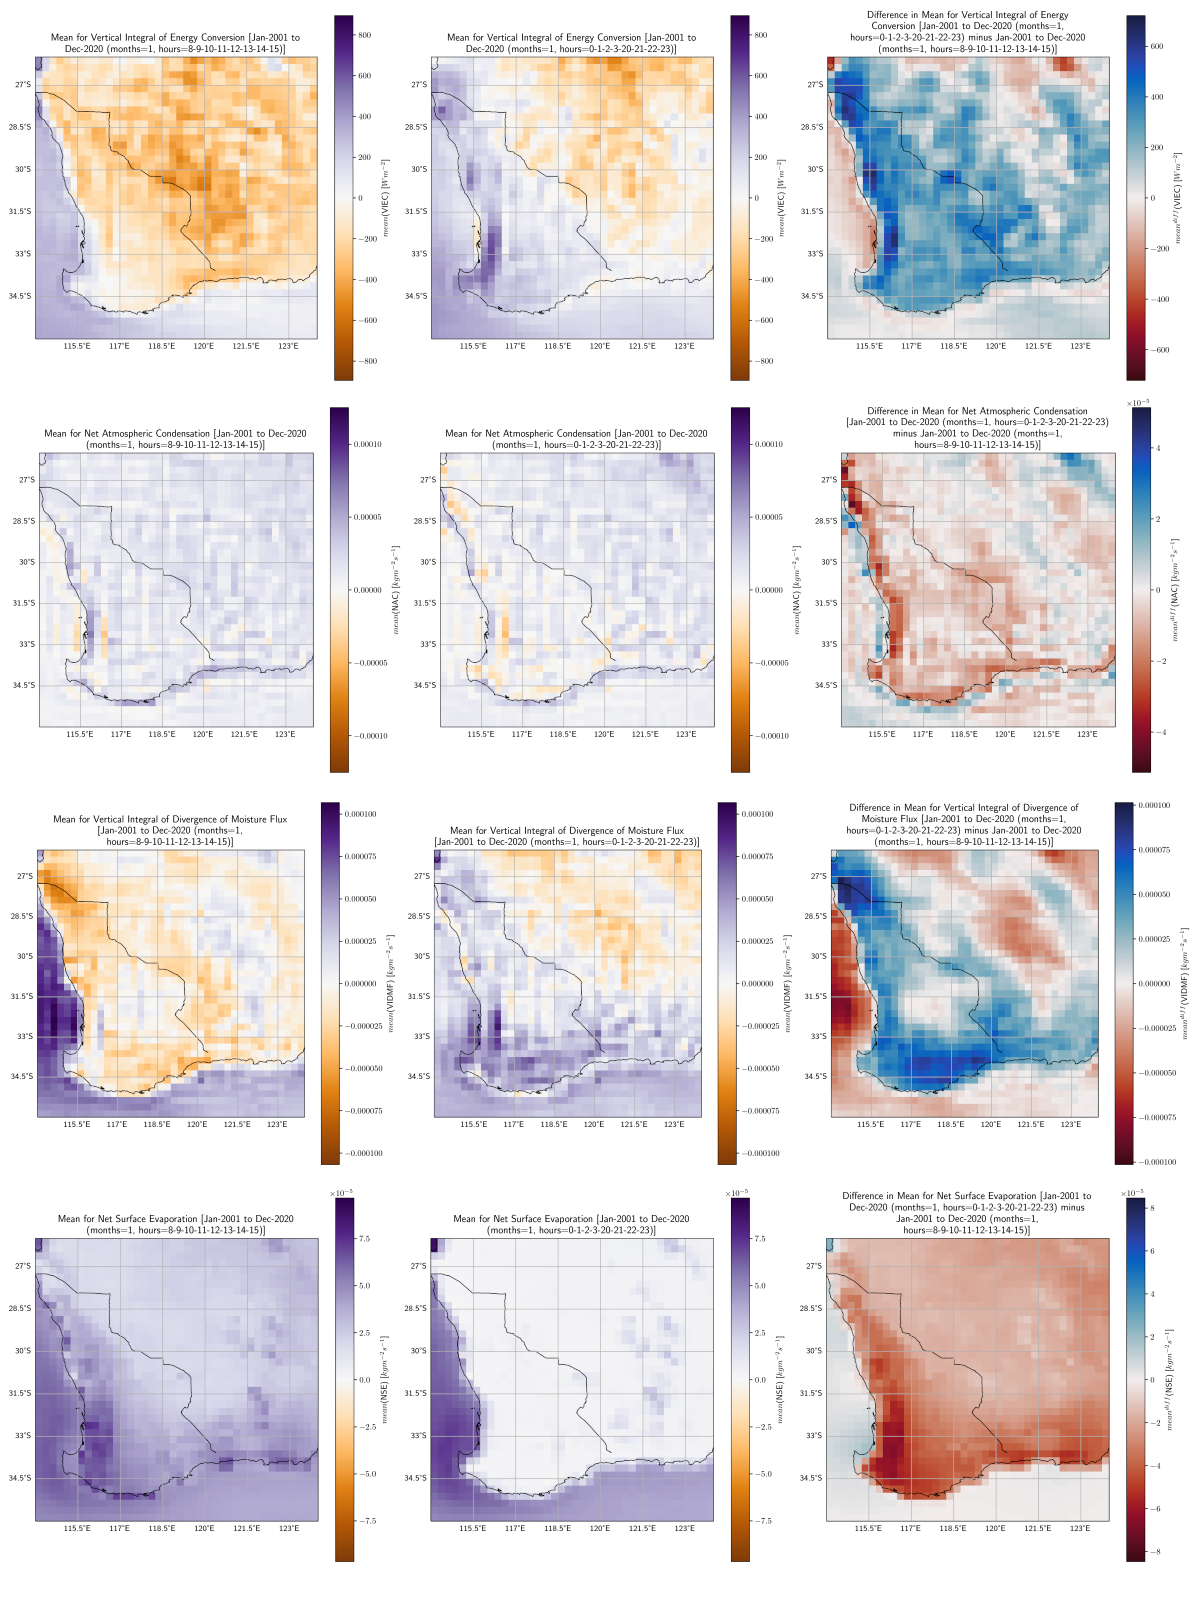
\includegraphics[width=0.9\textwidth]{wa_jan_comb_1_unmarked.png}
	\caption[January means for selected variables 1 (unmarked)]{January mean daytime and nighttime values for \acs{VIEC}, \acs{NAC}, \acs{VIDMF} and \acs{NSE}.}
	\label{fig:wa_jan_comb_1_unmarked}
\end{figure}

\subsection{January means for selected variables 2 (unmarked)}

The use of coloured markings with thick outline in Figure~\ref{fig:wa_jan_comb_2} somewhat distorts perception of the trends. For an undistorted view, see the January mean values for \ac{WS100}, \ac{dWS100}, \ac{MSLP} and \ac{T2} in Figure~\ref{fig:wa_jan_comb_2_unmarked}.

\begin{figure}[!htp]
	\centering
	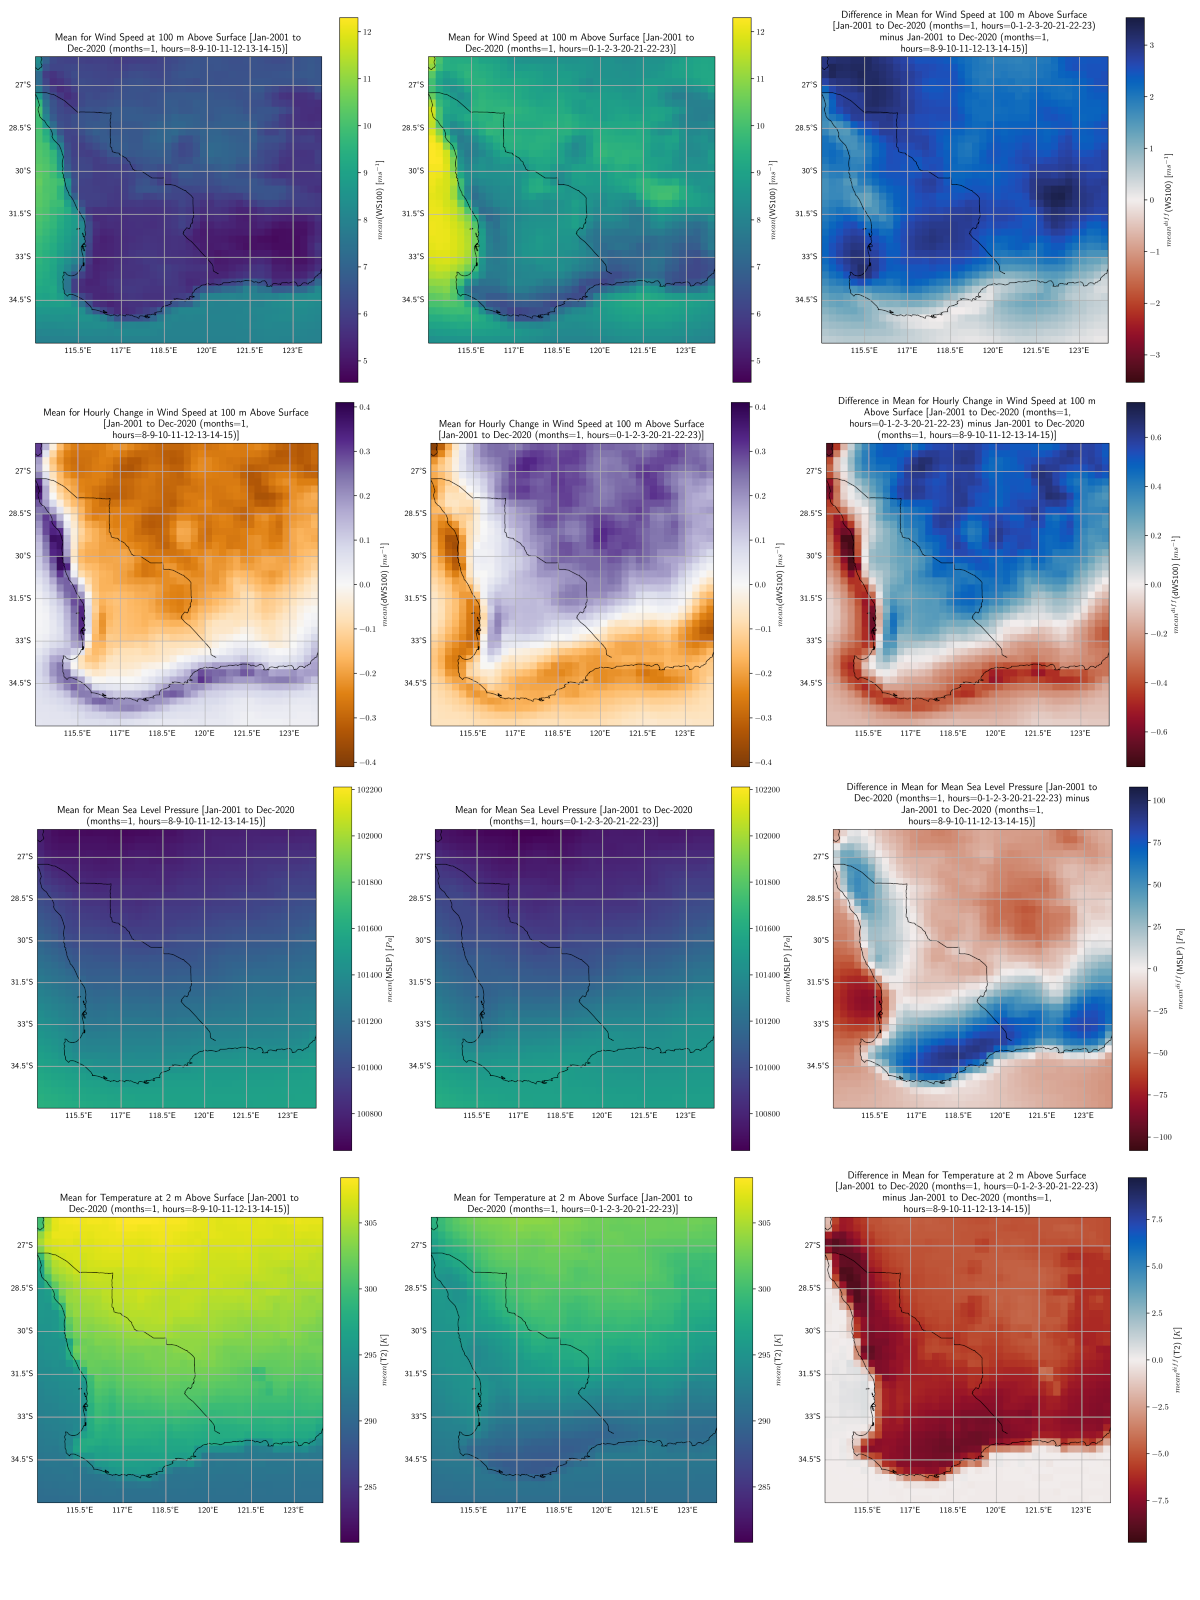
\includegraphics[width=0.9\textwidth]{wa_jan_comb_2_unmarked.png}
	\caption[January means for selected variables 2 (unmarked)]{January mean daytime and nighttime values for \acs{WS100}, \acs{dWS100}, \acs{MSLP} and \acs{T2}.}
	\label{fig:wa_jan_comb_2_unmarked}
\end{figure}

\section{Full list of study variables}

Some of the key variables studied in this project were presented in Section~\ref{sec:method_var}. For a full list of variables used in this study, including those which were analysed but for which there were no significant findings, see Table~\ref{tab:vars_analysis}.

\newcolumntype{P}[1]{>{\centering\arraybackslash}p{#1}}
\begin{landscape}
	%	\pagestyle{empty} %% only if you want to remove silly headers on the side	
	\begingroup
	\renewcommand\arraystretch{1.33} % only applicable to this table because of group
	
	\begin{longtable}{P{2cm}P{3cm}P{13cm}}
		\caption[Full list of study variables]{A full list of variables which were analysed. Abbreviations for these variables as used in the report are provided, along with descriptions of each variable.} 
		\label{tab:vars_analysis} 
		\\ 
		\toprule 
		\multicolumn{1}{P{2cm}}{\textbf{Abbreviation}}
		& \multicolumn{1}{P{3cm}}{\textbf{Variable}}
		& \multicolumn{1}{P{15cm}}{\textbf{Description}}\\	
		\midrule
		\endfirsthead
		\midrule
		\multicolumn{1}{P{2cm}}{\textbf{Abbreviation}}
		& \multicolumn{1}{P{3cm}}{\textbf{Variable}}
		& \multicolumn{1}{P{15cm}}{\textbf{Description}}\\	
		\midrule	
		\endhead
		\midrule	
		\multicolumn{3}{l@{}}{(continued\ldots)}\\
		\endfoot
		\endlastfoot
		\acs{LSE} & Land Surface Elevation & Units in $m$. Elevation of the land surface above sea level. Obtained by converting from ERA5 geopotential data using the MetPy Python library \citep{metpy}. \\
		\acs{SSGO} & Slope of Sub-Gridscale Orography & Dimensionless. Represents slopes of orographic features such as mountains and hills which are present down to a scale of 1 km. Flat surfaces have value 0 while vertical cliffs have value 1. \\ \midrule
		\acs{MLAI} & Mean Leaf Area Index & Dimensionless. The \ac{LAI} index for a grid cell is the total leaf area divided by ground area of that cell. \ac{MLAI} is the mean of this over the study period. This was the main metric used in assessing vegetation cover and vegetation cover change.  \\
		\acs{MFAPAR} & Mean Fraction of Photosynthetically Absorbed Radiation & Dimensionless. The \ac{FAPAR} for a grid cell is the fraction of radiation between 400-700 nm wavelength absorbed within that cell. \ac{MFAPAR} is the mean of this over the study period. This was a supplementary metric used in assessing vegetation cover and vegetation cover change. \\ \midrule
		\acs{BLH} & Boundary Layer Height & Units in $m$. Height of the depth of air for which surface effects are significant. This was used to assess level of convective mixing and likelihood fo cloud formation. \\
		CAPE & Convective Available Potential Energy & Units in $J kg^{-1}$. Work which would be performed on an air parcel if it rose through the atmosphere. This was used to indicate atmospheric stability. The more positive the more air will rise, the more negative the more air will sink. \\
		\acs{CBH} & Cloud Base Height & Units in $m$. Height for base of lowest cloud. This was used to assess how height of cloud formation may affect atmospheric circulations. \\
		FA & Forecast Albedo & Dimensionless. Fraction of short-wave radiation reflected from surface. This was used to assess how reflectivity of different land cover affects the surface energy balance. \\
		\acs{MSLP} & Mean Sea Level Pressure & Units in $Pa$. Pressure of atmosphere adjusted to sea level. This is one of the main variables affecting wind. High values typically coincide with calm conditions while low values coincide with windy. This was also used to identify synoptic features. \\
		\acs{NAC} & Net Atmospheric Condensation & Units in $kg m^{-2} s^{-1}$. Condensation minus evaporation in atmosphere (does not include surface). Positive values indicate more cloud formation than cloud evaporation. Calculated using \ac{ERA5} data for \ac{TCWV}, \ac{NSE} and \ac{VIDMF} (see Appendix~\ref{sec:nac_derive}). This is one of the major factors affecting the partitioning of the atmospheric energy budget. \\
		\acs{NSE} & Net Surface Evaporation & Units in $kg m^{-2} s^{-1}$. Evaporation minus condensation at surface (does not include atmosphere). For vegetation, positive values indicate a greater amount of evapotranspiration than dew formation. Instantaneous values are approximated by averaging consecutive \ac{ERA5} accumulation values.\footnote{\ac{ERA5} parameters come in instantaneous and accumulation values. Instantaneous values are calculated for that point in time at each hour whereas accumulation values represent a sum compiled over the course of the previous hour window. \ac{NSE}, \ac{SLHF} and \ac{SSHF} are accumulation values whereas the remainder are instantaneous. Averages for these variables were computed to approximate "instantaneous" values in order to allow an apples to apples comparison.} \\
		\acs{SLHF} & Surface Latent Heat Flux & Units in $W m^{-2}$. Rate at which energy at the surface is being used for evapotranspiration. Instantaneous values are approximated by averaging consecutive \ac{ERA5} accumulation values (see \ac{NSE} footnote). \\
		\acs{SSHF} & Surface Sensible Heat Flux & Units in $W m^{-2}$. Rate at which energy at the surface is being used to induce convection and warming of the air mass above it. Instantaneous values are approximated by averaging consecutive \ac{ERA5} accumulation values (see \ac{NSE} footnote). \\
		\acs{T2} & Temperature at 2 m Above Surface & Units in $K$. This is one of the major factors affecting the partitioning of the atmospheric energy budget. \\
		\acs{TCC} & Total Cloud Cover & Dimensionless. Fraction of grid cell covered by cloud. \\
		\acs{TCCLW} & Total Column Cloud Liquid Water & Units in $kg m^{-2}$. Total cloud liquid content averaged over grid cell. Does not include rain water droplets. \\
		\acs{TCWV} & Total Column Water Vapour & Units in $kg m^{-2}$. Total amount of water vapour averaged over grid cell. Often referred to as precipitable water (PW). \\
		\acs{U10} & Zonal Component of 10 m Wind Velocity & Units in $m s^{-1}$. East-West component of wind velocity at 10 m above surface. Positive values indicate that wind has a westerly component (blowing \textit{to} the east). \\
		\acs{U100} & Zonal Component of 10 m Wind Velocity & Units in $m s^{-1}$. East-West component of wind velocity at 100 m above surface. Positive values indicate that wind has a westerly component (blowing \textit{to} the east). \\
		\acs{V10} & Meridional Component of 10 m Wind Velocity & Units in $m s^{-1}$. North-South component of wind velocity at 10 m above surface. Positive values indicate that wind has a southerly component (blowing \textit{to} the north). \\
		\acs{V100} & Meridional Component of 100 m Wind Velocity & Units in $m s^{-1}$. North-South component of wind velocity at 100 m above surface. Positive values indicate that wind has a southerly component (blowing \textit{to} the north). \\
		\acs{VIDMF} & Vertical Integral of Divergence of Moisture Flux & Units in $kg m^{-2} s^{-1}$. The average rate at which water vapour in a grid cell is leaving to neighbouring grid cells.\footnote{Note that \ac{ERA5} has a similarly named parameter called \ac{VIMF} which is an accumulation rather than instantaneous parameter, but with the crucial difference that "moisture" in this variable refers to the total of water vapour, cloud liquid and cloud ice. The ERA5 documentation for \ac{VIDMF} also refers to "moisture" and it is not apparent that this actually uses a different definition where it only includes water vapour, but this was indeed confirmed to be the case via correspondence with \ac{ECMWF} specialist support.} Positive values indicate water vapour is diverging (leaving grid cell) while negative values indicate water vapour is converging (entering grid cell). \\
		\acs{VIEC} & Vertical Integral of Energy Conversion & Units in $W m^{-2}$. Rate at which energy is being converted from internal plus potential energy into kinetic energy.\footnote{By \ac{ERA5} definitions, internal energy refers to the microscopic energy of the air molecules excluding latent energy (this is treated as a separate part of the atmospheric energy budget) which may be different to definitions used in chemistry. Potential energy here refers to macroscopic gravitational potential energy (as opposed to internal air pressure within the grid cell, as this is implicitly accounted for within internal energy). Kinetic energy refers to kinetic energy from the \textit{horizontal} motion of air masses.} Negative values indicate kinetic energy conversion into internal plus potential energy. \\
		\acs{VIKE} & Vertical Integral of Kinetic Energy & Units in $J m^{-2}$. Total kinetic energy from the \textit{horizontal} motion of air masses through the grid cell, averaged over the grid cell. This was used to study how land cover change affects partitioning in the atmospheric energy budget. \\
		\acs{VIPILE} & Vertical Integral of Potential, Internal and Latent Energy & Units in $J m^{-2}$. Total of gravitational potential energy, internal energy and latent energy (see footnote for \ac{VIEC}). This constitutes the total atmospheric energy budget minus kinetic energy. This was used to study how land cover change affects partitioning in the atmospheric energy budget. \\
		\acs{WS10} & Wind Speed at 10 m Above Surface & Units in $m s^{-1}$. Scalar quantity for wind speed at 10 m above surface. \\
		\acs{WS100} & Wind Speed at 100 m Above Surface & Units in $m s^{-1}$. Scalar quantity for wind speed at 100 m above surface. This is the quantity most directly relevant for wind energy generation. \\
		\acs{WV10} & Wind Velocity at 10 m Above Surface & Units in $m s^{-1}$. Vector quantity for wind velocity at 10 m above surface. \\
		\acs{WV100} & Wind Velocity at 100 m Above Surface & Units in $m s^{-1}$. Vector quantity for wind velocity at 100 m above surface. This quantity is also directly relevant for wind energy generation and furthermore highlights how wind direction changes. \\ \midrule
		d\{VAR\} & Hourly Change in \{VAR\} & Units vary. Change in the value for each of the above \ac{ERA5} or \ac{ERA5}-derived values, as compared with its value in the previous hour. This was used to study how the rate of change of a variable was correlated with land cover change. \\ \midrule
		\acs{C10} & Weibull Scale Parameter for 10 m Wind Speed & Units in $m s^{-1}$. Scale parameter for the Weibull distribution fit to the wind speed at 10 m above surface. The empirical Weibull fit was obtained using the equations of \citep{justus1977}. \\
		\acs{C100} & Weibull Scale Parameter for 100 m Wind Speed & Units in $m s^{-1}$. Scale parameter for the Weibull distribution fit to the wind speed at 100 m above surface. The empirical Weibull fit was obtained using the equations of \citep{justus1977}. \\
		\acs{EROE100} & Expected Rate of 100 m Wind Speed Exceeding 42.5 m/s & Dimensionless. The \textit{expected} rate for wind speed at 100 m exceeding 42.5 m/s, which in practice is the typical wind speed which wind turbines can last 10 mins in before failure \citep{chen2015, chen2016, ge_web}. This is the \textit{expected} rate calculated from the tail of the Weibull distribution fit rather than the actual observed rate of exceedance. \\
		\acs{K10} & Weibull Shape Parameter for 10 m Wind Speed & Dimensionless. Shape parameter for the Weibull distribution fit to the wind speed at 10 m above surface. The empirical Weibull fit was obtained using the equations of \citep{justus1977}. \\
		\acs{K100} & Weibull Shape Parameter for 100 m Wind Speed & Dimensionless. Shape parameter for the Weibull distribution fit to the wind speed at 100 m above surface. The empirical Weibull fit was obtained using the equations of \citep{justus1977}. \\
		$mean$(\acs{WS10}) & Mean of 10 m Wind Speed & Units in $m s^{-1}$. Mean of wind speed at 10 m above surface. This is roughly equivalent to the mean of the mean diurnal profile for \ac{WS10} (see Section~\ref{ssec:mean_commute}). \\
		$mean$(\acs{WS100}) & Mean of 100 m Wind Speed & Units in $m s^{-1}$. Mean of wind speed at 10 m above surface. This is roughly equivalent to the mean of the mean diurnal profile for \ac{WS100} (see Section~\ref{ssec:mean_commute}). \\
		$std$(\acs{WS10}) & Standard Deviation of 10 m Wind Speed & Units in $m s^{-1}$. Standard deviation of wind speed at 10 m above surface. This is used with \ac{K10} to analyse how the variability in wind speed changes along with land cover. \\
		$std$(\acs{WS100}) & Standard Deviation of 100 m Wind Speed & Units in $m s^{-1}$. Standard deviation of wind speed at 10 m above surface. This is used with \ac{K100} to analyse how the variability in wind speed changes along with land cover. \\
		\acs{TGCF100} & Typical Gross Capacity Factor for 100 m Turbine & Dimensionless. Gross capacity factor which a typical 2.5 MW turbine with 100 m hub height would have had over the study period. This was computed by first averaging the power curves for similar 2.5 MW turbines from Vestas, Goldwind and GE Energy, then computing the energy generation for each hour in the study period using \ac{ERA5} data for the wind speed at 100 m above surface (see Section~\ref{ssec:method_wsd}). \\ \bottomrule
	\end{longtable}
	
	\endgroup
\end{landscape}

\section{Assimilation cycle artefacts in ERA5}
\label{sec:artefact}

\subsection{Artefacts in TCWV}

The hourly mean results for \ac{dTCWV} at hours 0600 \ac{LT} (2200 UTC) and 1800 \ac{LT} (1000 UTC) indicate a discontinuous change in \ac{TCWV} (not shown). These values represent the change in \ac{TCWV} from 2100-2200 UTC and 0900-1000 UTC respectively. The humidity (and by extension \ac{TCWV}) values in ERA5 are known to have a mismatch between the end of one assimilation cycle and the beginning of the next, which happen at exactly these time windows \citep{ecmwf}.

\subsection{Artefacts inherited by NAC}

Because the \ac{NAC} value at hour i is derived using the \ac{TCWV} values at hours i-1 and i+1 (see Appendix~\ref{sec:nac_derive}), the \ac{NAC} value at hours 0500-0700 \ac{LT} and 1700-1900 \ac{LT} inherit these discontinuities (see Figure~\ref{fig:wa_dnac_artefact}). These discontinuities are not observed for any of the other variables which \ac{NAC} is derived from (\ac{NSE} and \ac{VIDMF}).

\begin{figure}[!htp]
	\centering
	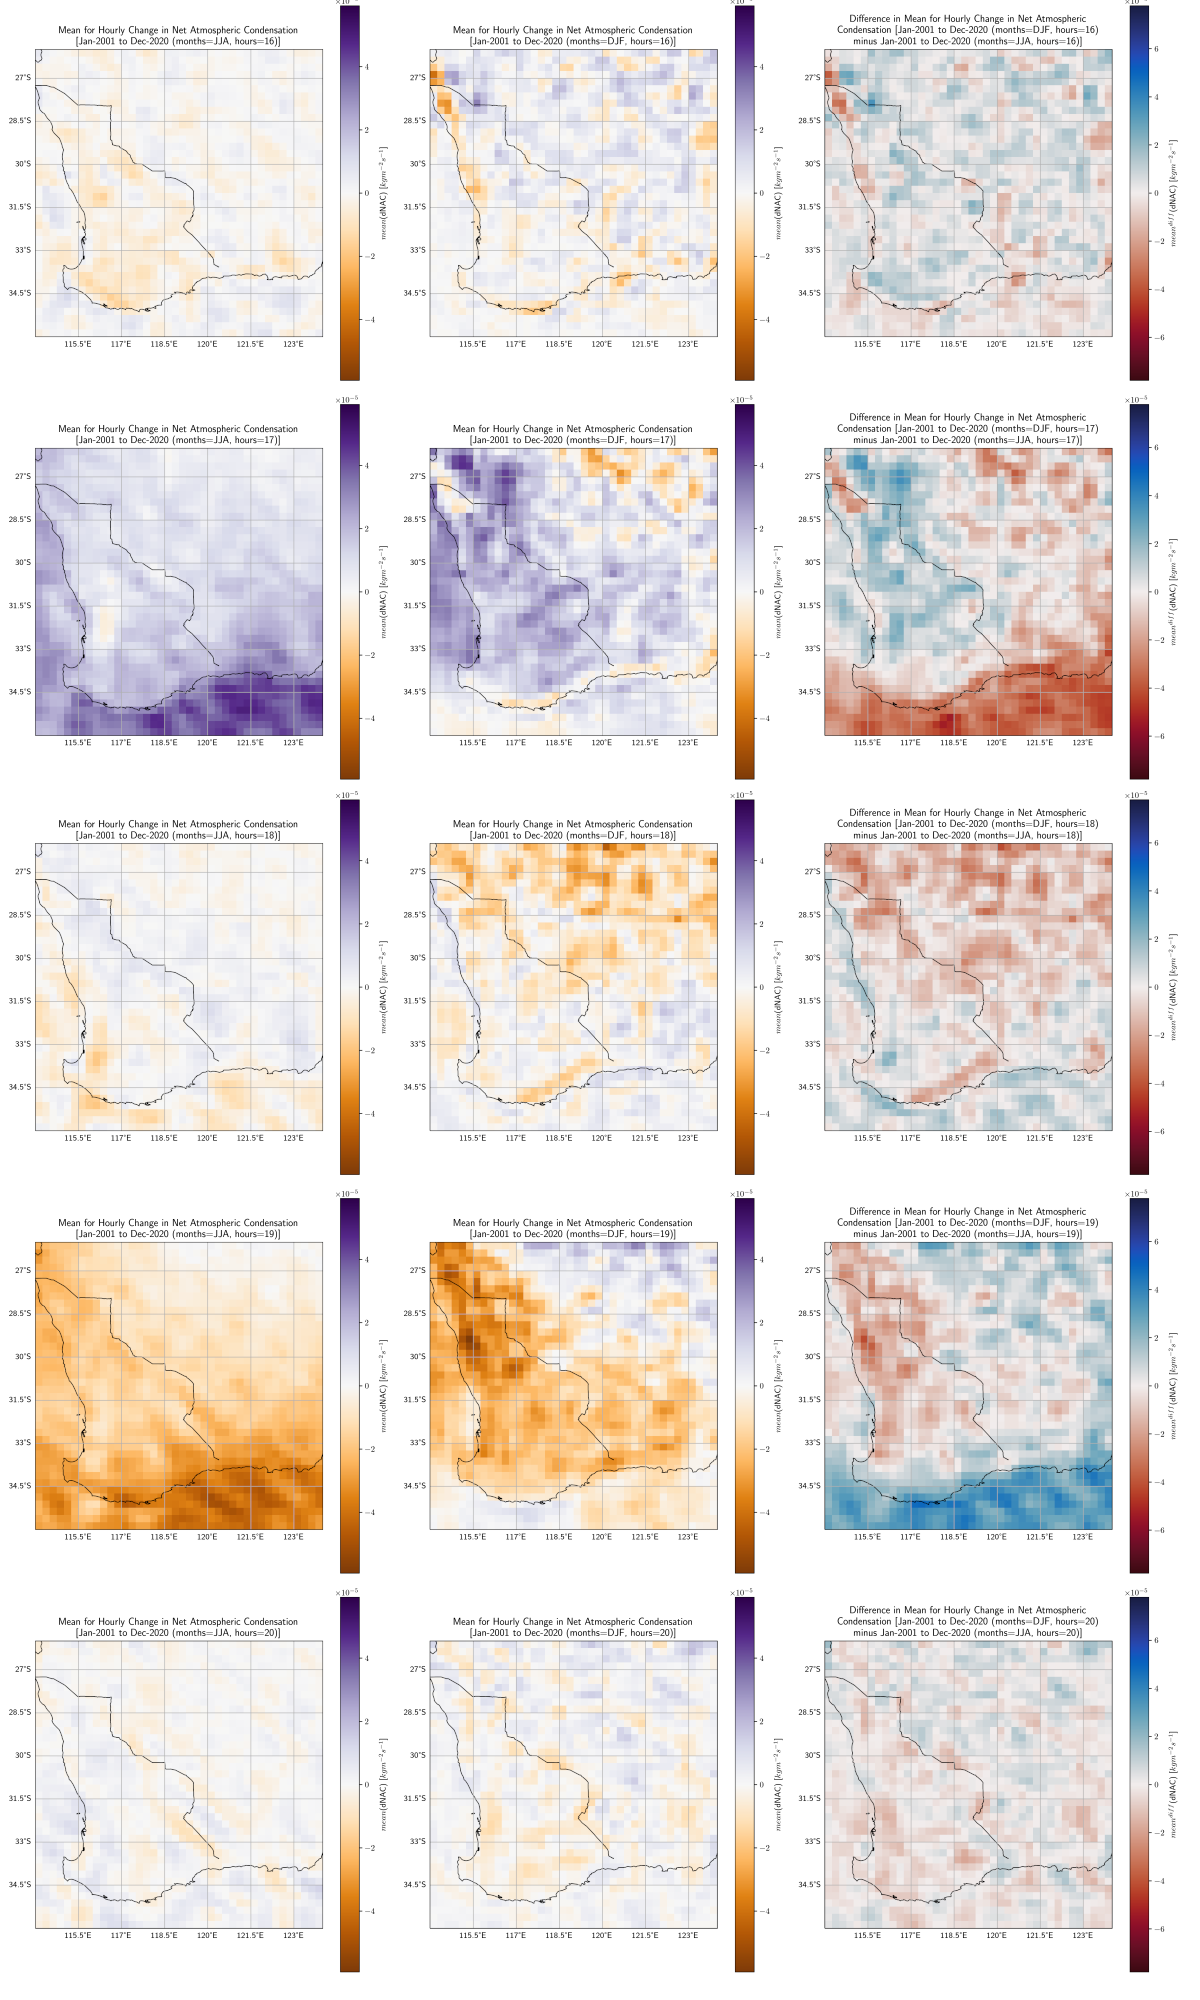
\includegraphics[width=0.75\textwidth]{wa_dnac_artefact.png}
	\caption[1600-2000 means for dNAC (artefacts)]{1600-2000 mean \ac{JJA} and \ac{DJF} values for \acs{dNAC}. 1600 and 2000 means are in line with means in remaining hours. Artefacts inherited from \ac{TCWV} assimilation cycles show opposite trends at 1700 and 1900.}
	\label{fig:wa_dnac_artefact}
\end{figure}

\subsection{Results relatively unaffected}

Figure~\ref{fig:wa_dnac_artefact} shows how this leads to unusually large \ac{dNAC} means from 1700-1900 \ac{LT}. But importantly, the increases at 1700 \ac{LT} are offset by a spatially correlated decrease of comparable magnitude at 1900 \ac{LT}. Analogous results were found between 0500-0700 \ac{LT} (not shown). So the means computed over the course of this project should be relatively unaffected. This applies even for the diurnal comparison where means were computed over a subset of hours, since daytime and nighttime hours were defined as 0800-1500 \ac{LT} and 2000-0300 \ac{LT} respectively (see Section~\ref{ssec:method_diurnal_seasonal}), which falls outside of the hours with artefacts. This does mean, however, that \ac{MDP} statistics apart from the mean (hour of maximum, hour of minimum, maximum, minimum and range) need to be interpreted with care when it comes to \ac{TCWV}, \ac{dTCWV}, \ac{NAC} and \ac{dNAC}. 

\subsection{Other affected variables}

None of the other key study variables apart from \ac{FA} were found to have similarly obvious assimilation cycle discontinuities, but \ac{FA} was only used for one result (Figure~\ref{fig:wa_stats_seasonal_2}) which was a mean over all hours of the day so results should still be relatively unaffected.

\section{Other focus regions in original project scope}
\label{sec:other_regions}

The original project scope included results for \ac{CA} and \ac{NB} but time did not allow for detailed analysis, discussion and presentation of these results. Included below is a summary for each of these regions, as well as the selected periods for the similar comparison. This may be used for future research.

\subsection{General}

\subsubsection{Periods for diurnal and seasonal comparison}

For all focus regions, the diurnal and seasonal comparisons were performed over the period from Jan-2001 to Dec-2020 (inclusive). The GLASS products derived from \ac{MODIS}, the more advanced instrument, begin around Mar-2000, with the \ac{LAI} dataset ending Dec-2021 while the \ac{FAPAR} dataset ends Dec-2020 (at the time of writing). As averages starting from Mar-2000 and ending Dec-2020 would have skewed weightings for the months of January and February, we elected to use Jan-2001 as the period start instead.

\subsubsection{Wet and dry months}

Based on historical precipitation climatology, we have selected the months representing the wet and dry seasons for each region as being:
\begin{itemize}
	\item \ac{WA}: June, July, August (JJA) and December, January, February (DJF) respectively
	\item \ac{CA}: May to October (5-6-7-8-9-10) and November to April (1-2-3-4-11-12) respectively
	\item \ac{NB}: January to June (1-2-3-4-5-6) and July to December (7-8-9-10-11-12)
\end{itemize}

\subsubsection{Daytime and nighttime hours}

The local timezones for \ac{WA}, \ac{CA} and \ac{NB} are UTC+8, UTC-6 and UTC-3 respectively\footnote{The focus region for \ac{NB} spans across 35 degrees of longitude, so it actually covers multiple local timezones and over more than 2 hours of local solar timezones (15 degrees per hour). We have selected UTC-3 here because this is close to the local solar timezone for the midpoint of this region.}. Where comparisons between daytime and nighttime hours have been made, the average values for hours from 8 am to 3 pm local time\footnote{Unless otherwise stated, all times in this report are expressed in local time, and hour endpoints are inclusive.} (8-9-10-11-12-13-14-15) have been selected as representative of daytime, while the average values for hours from 8 pm to 3 am local time (0-1-2-3-20-21-22-23) have been selected as representative of nighttime.

\subsubsection{Orography}

The orography for each focus region is displayed in Figure~\ref{fig:orog}.

\begin{figure}[!ht]
	\centering
	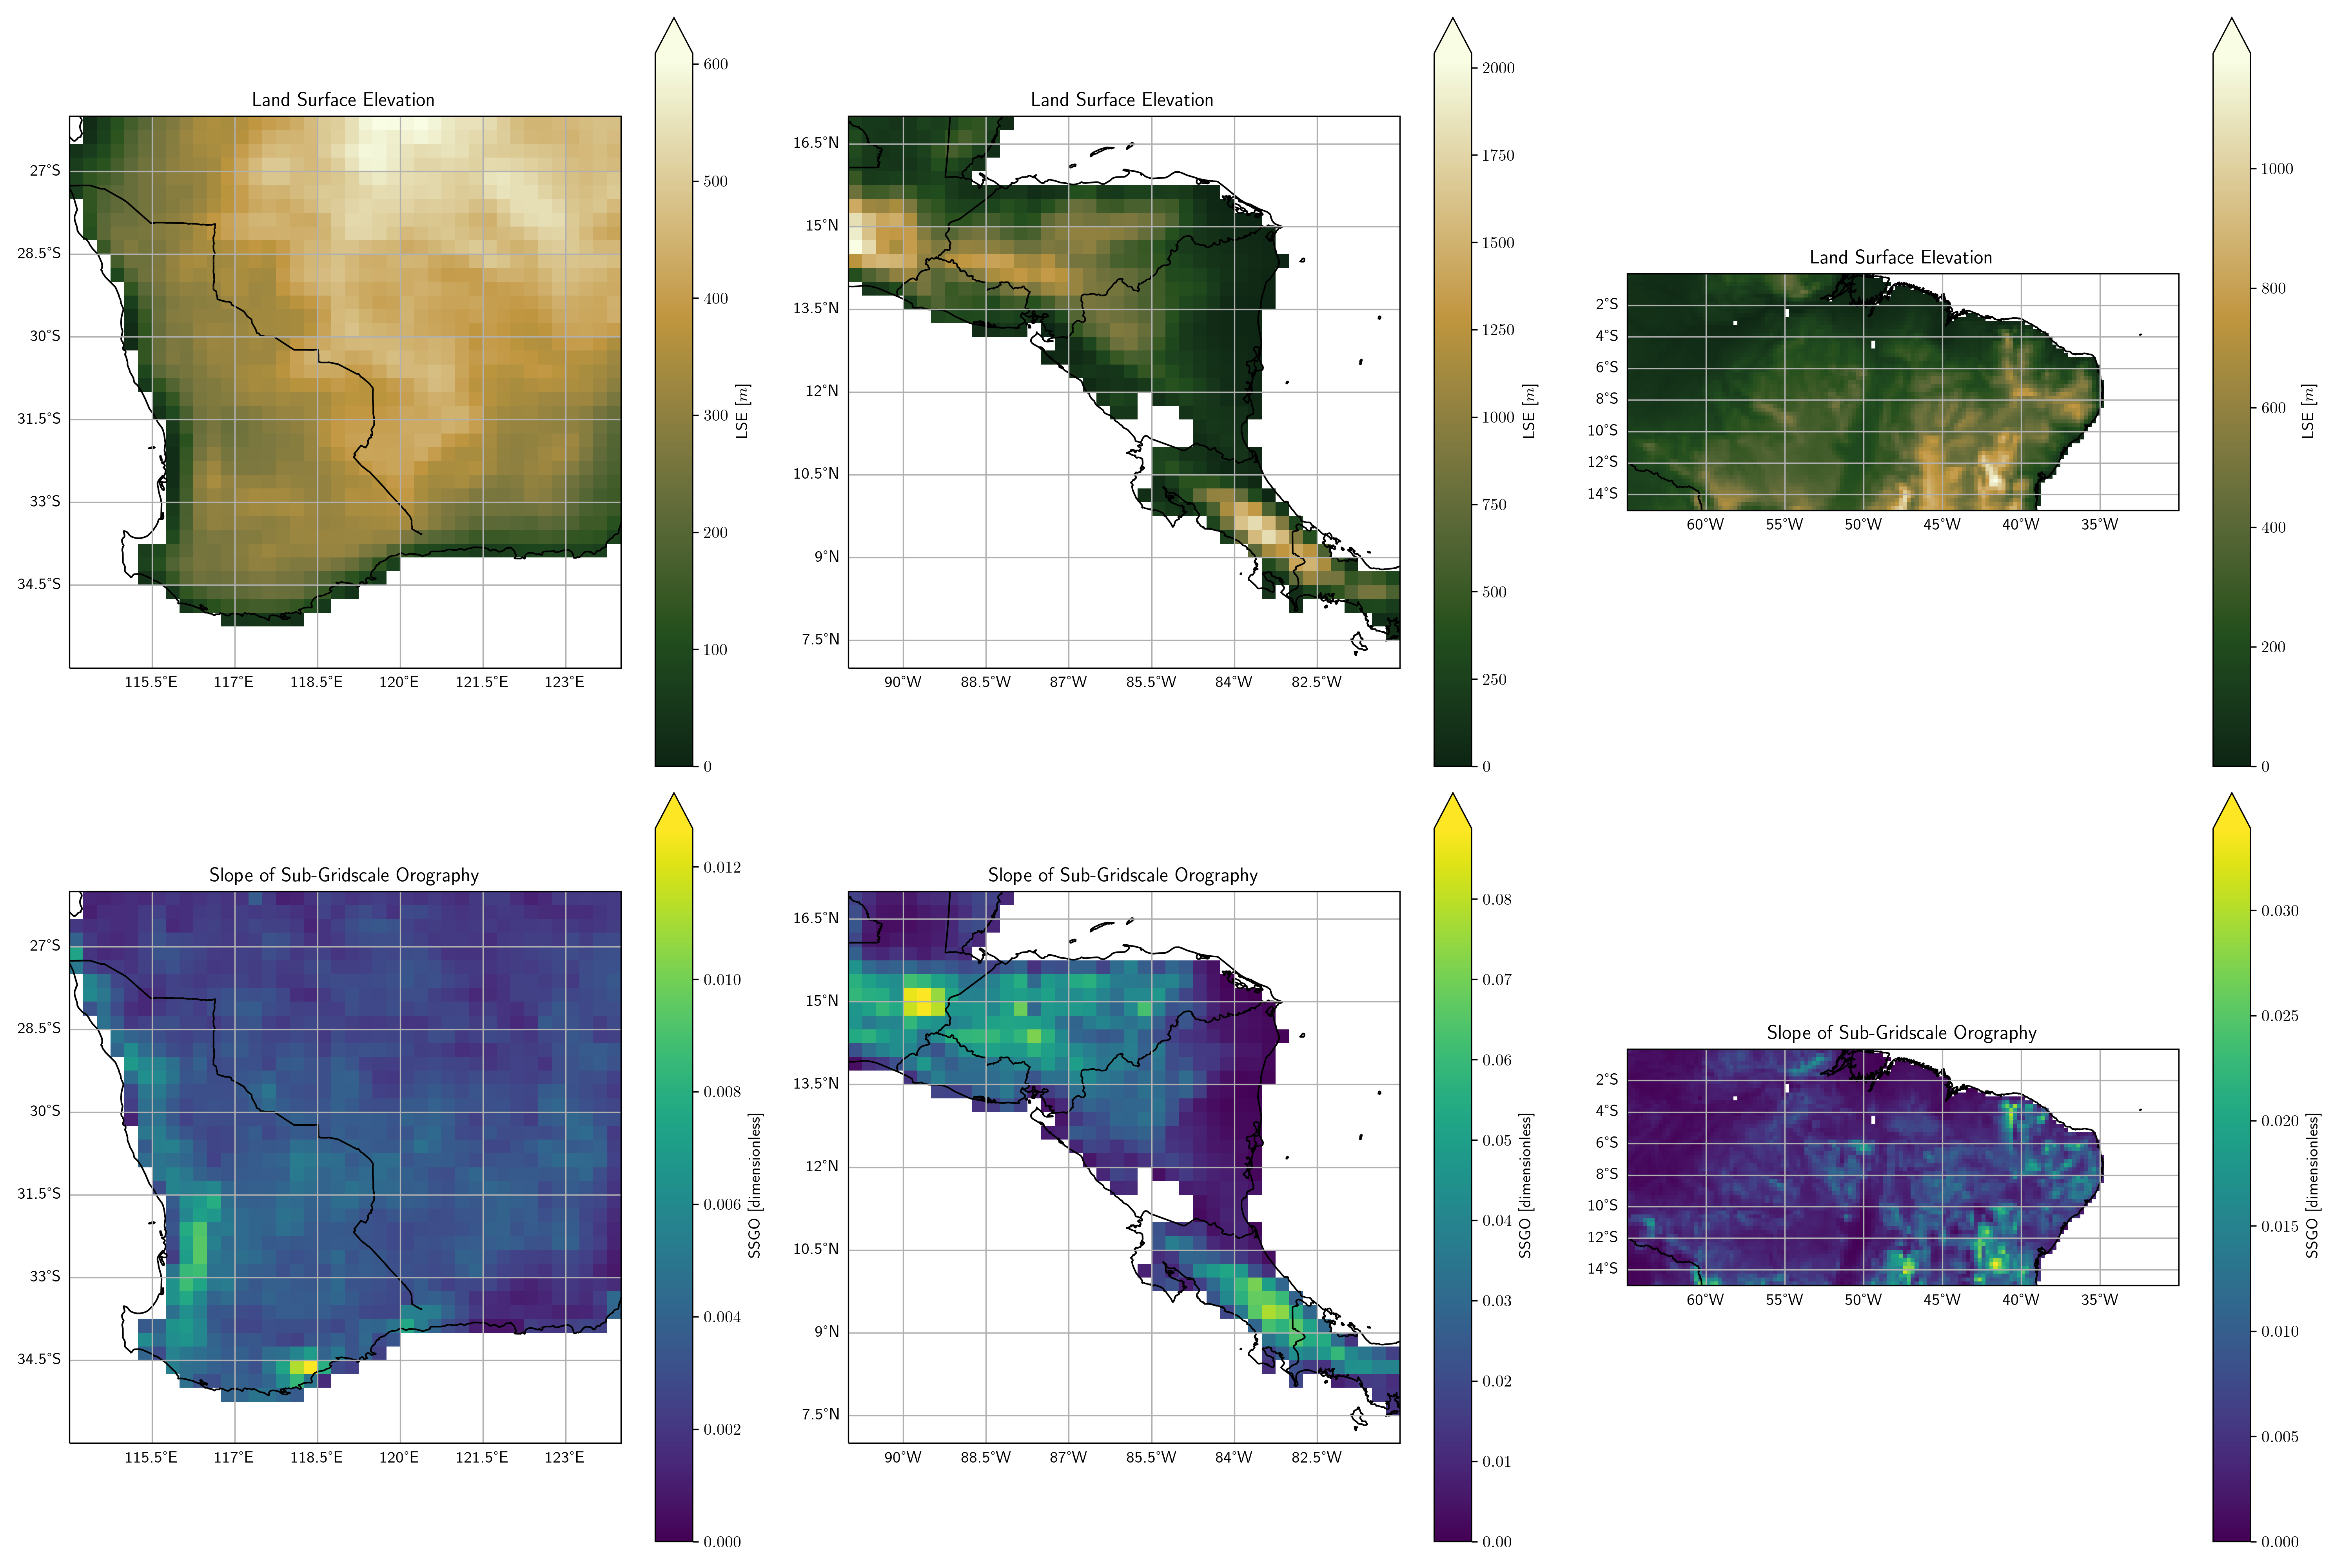
\includegraphics[width=0.9\textwidth]{orog.png}
	\caption[Orography for all focus regions]{Top row: \acf{LSE} for each region. Bottom row: \acf{SSGO} for each region. From left to right: \acl{WA}, \acl{CA}, \acl{NB}.}
	\label{fig:orog}
\end{figure}

\subsection{Central America}

\begin{figure}[!ht]
	\centering
	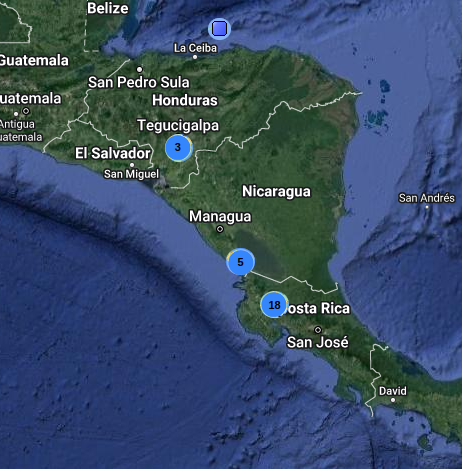
\includegraphics[width=0.75\textwidth]{maps_twp_ca}
	\caption[Central America Map]{Satellite image displaying Central America focus region from 91$^\circ$W to 81$^\circ$W longitude and 17$^\circ$S to 7$^\circ$S latitude \citep{maps_ca}. Markers indicating positions and number of wind farms have been edited on using data from \citep{twp_hd, twp_nc, twp_cr}.}
	\label{fig:maps_twp_ca}
\end{figure}

\subsubsection{Description of region}

We selected the part of \ac{CA} which runs (North to South) from El Salvador and Honduras to Nicaragua to Costa Rica (91$^\circ$W to 81$^\circ$W longitude and 17$^\circ$S to 7$^\circ$S latitude; see Figure~\ref{fig:maps_twp_ca}) because there existed spatially opposing trends in vegetation change. These countries had historically comparable rates of deforestation, but Costa Rica shifted towards reforestation due to policy changes in the 1990s whereas deforestation has continued in Honduras and Nicaragua. The western coastlines for El Salvador, Nicaragua and Costa Rica (where agriculture is concentrated) also have comparable cardinal orientations.

Being located near the equator, annual temperature variation at these locations are relatively minor. This is useful because it provides a comparison where one of the main variables affecting wind flow is relatively controlled for. Furthermore, the entire focus region is on the order of 1000 km, so synoptic weather features (which have a characteristic scale of this order) are less likely to produce contrasting effects over the different subregions.

\subsubsection{Significance of results from this region}

Wind farms are concentrated on agricultural land along the western coast where there are plans for continued development. But as in the case of \ac{WA}, the value of this focus region isn't necessarily in its direct implications for existing wind farms in the area, but in that it may yield some insights into the principles between land cover change and surface winds, which may then have broader implications for wind energy generation in general.

\subsubsection{Study periods}
\label{sssec:period_seas_ca}

\paragraph{Selected periods}

For \ac{CA}, the selected periods for the similar comparison was from Jan-2002 to Dec-2006 and from Jan-2014 to Dec-2018 (see Figure~\ref{fig:ca_ind}).

\begin{figure}[!htp]
	\centering
	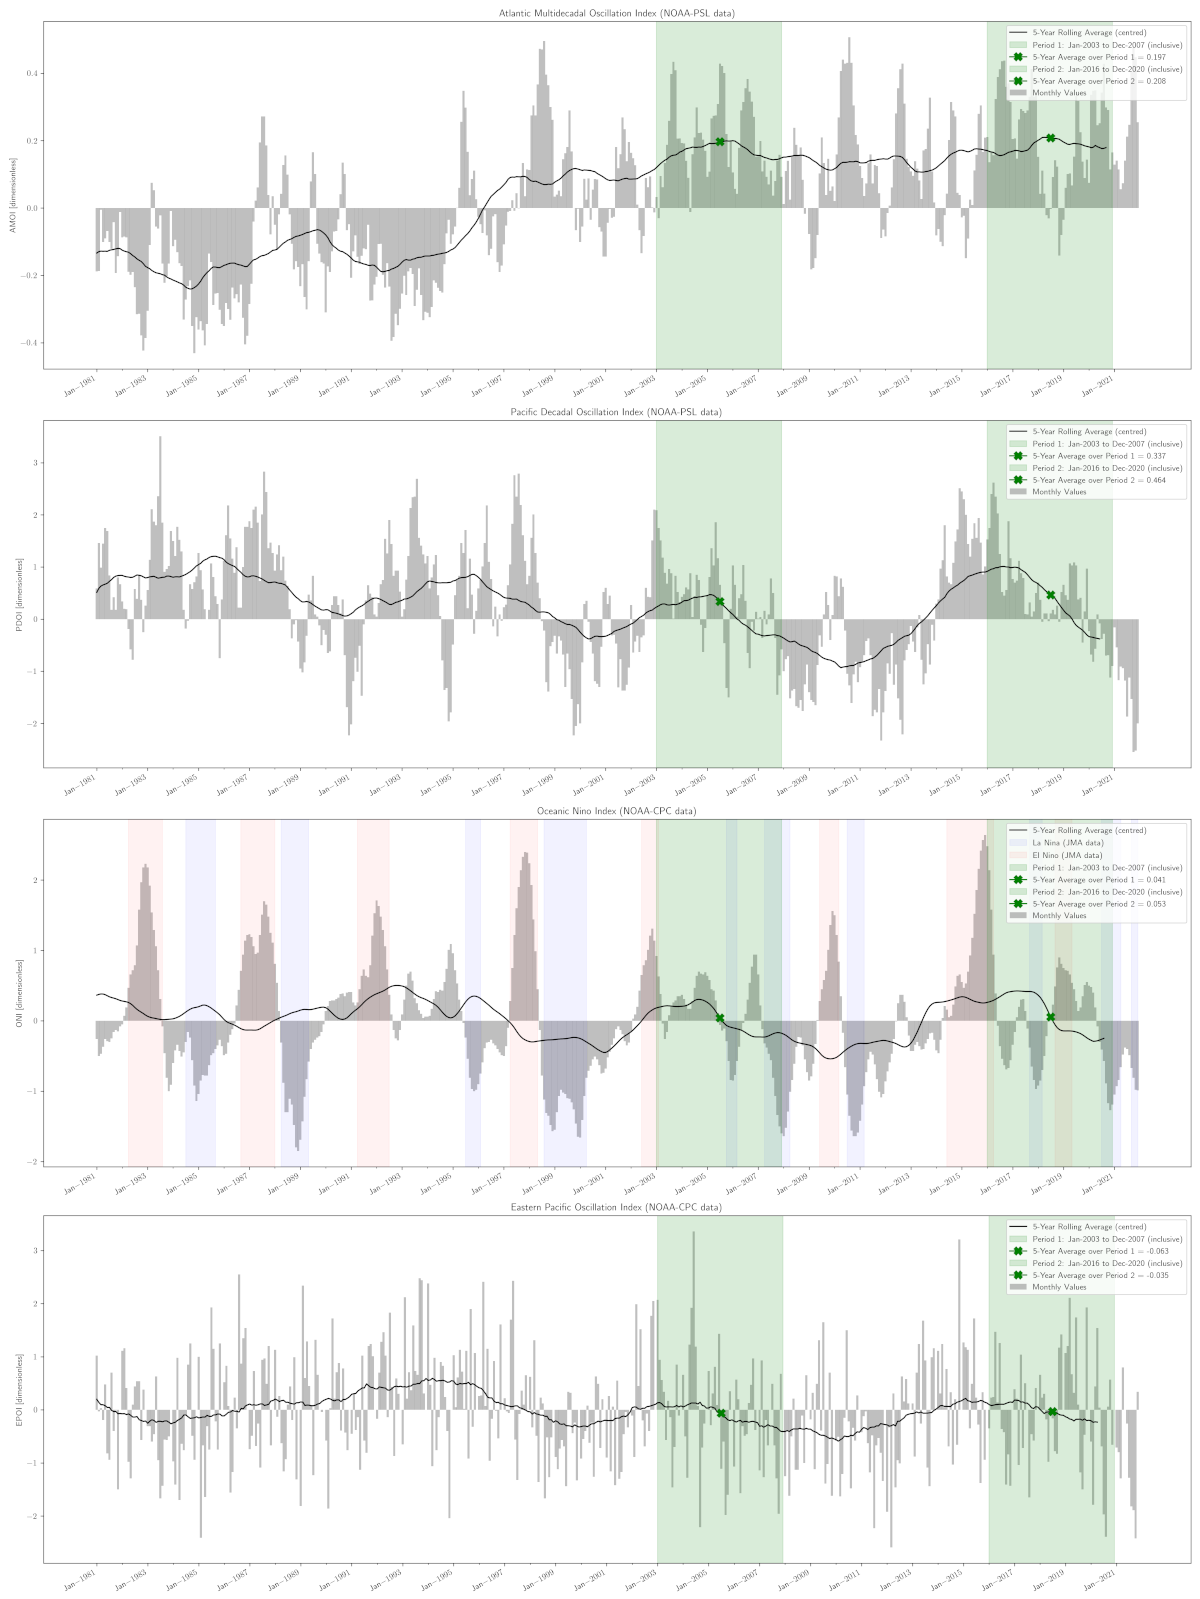
\includegraphics[width=0.9\textwidth]{ca_ind.png}
	\caption[CA's and SA's relevant climate indices for similar comparison]{\ac{NOAA} climate indices for climate drivers in \ac{CA}. Green shading highlights selected periods. Blue and red shading highlight La Nina and El Nino events respectively.}
	\label{fig:ca_ind}
\end{figure}

\paragraph{Very similar values and trends in climate indices}

The pair of Jan-2002 to Dec-2006 and Jan-2014 to Dec-2018 was deemed most appropriate since these periods had comparable averages in relevant climate indices and appear to span across the same phase of the relevant atmospheric oscillations. This was true for all of the relevant indices: \ac{AMOI}, \ac{PDOI}, \ac{ONI} (for \ac{ENSO}), and the \ac{EPOI}. The \ac{AOI} and \ac{NAOI} over these periods (not shown) also appeared to span across the same phase but had 5-year averages with slightly higher disparities (but these disparities were nevertheless small in terms of the characteristic size of the oscillations). The \ac{DMI} and the \ac{AAOI} (not shown) over these periods, on the other hand, were considerably different, but these were assumed not to be a major factor due to the distance of the Indian Ocean and Antarctica from the Americas\footnote{Significant effects due to teleconnections are theoretically possible but we have assumed this isn't the case here}.

\paragraph{Summary of El Nino-Southern Oscillation events}

The similarity between these periods is particularly remarkable because even the monthly values and 5-year averages for the \ac{ONI} (which has irregular oscillations) display a similar time evolution pattern. Both periods begin with the conclusion of an El Nino event and end past halfway into an La Nina event, and fully covers another La Nina event in between. The period from Jan-2014 to Dec-2018 contains an additional El Nino event not found in the period from Jan-2002 to Dec-2006 but this appears to mostly be a technicality with the definition of an El Nino event. A look at the monthly values reveals a spike in the \ac{ONI} which could have qualified as an El Nino event under slightly relaxed definitions. Furthermore, the monthly values between the starting El Nino event and ending La Nina event are almost mirror images of each other.

\paragraph{Time difference between periods well suited for studying land cover change}

In the case of Costa Rica, although remote sensing indicates that the rate of forest cover increase here was highest during the 1990s, leaf area index data derived from the \ac{AVHRR} instrument (not shown) for this region showed considerable noise and disagreement with \ac{MODIS} (the more advanced instrument). Given these factors, this set of study periods was also desirable because it was completely contained within the \ac{MODIS} coverage period. In addition to this, a land cover classification study by \citet{marx2017} using Landsat and \ac{UAV} data in lowland Costa Rica suggested an 11-year period for a pasture to transition into secondary forest, so a 13 year difference between selected periods corresponds well with our goals for studying the effects of \ac{LCC}. The change in \ac{MLAI} between these periods is displayed in Figure~\ref{fig:ca_lai_similar}.

\begin{figure}[!ht]
	\centering
	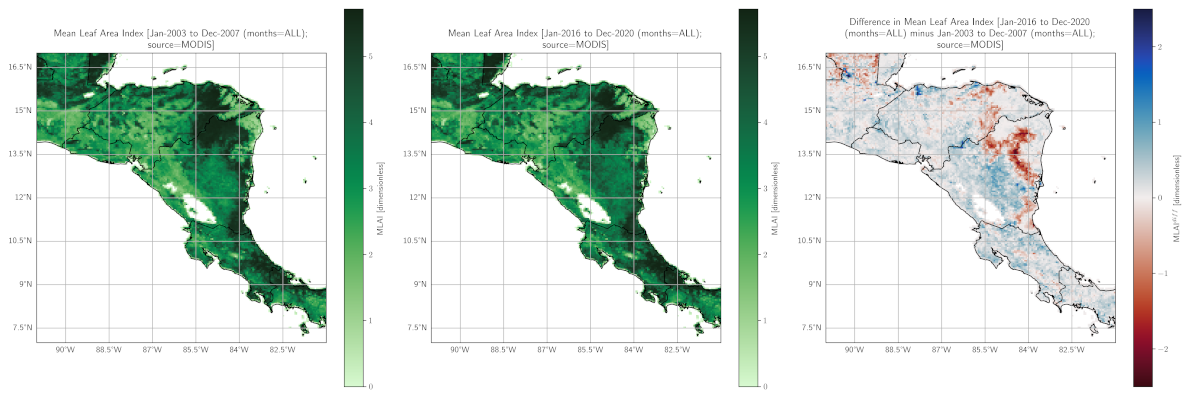
\includegraphics[width=0.9\textwidth]{ca_lai_similar.png}
	\caption[MLAI similar comparison for CA focus region]{\ac{MLAI} computed over each period in the similar comparison (left and middle), as well as the difference in these values between the two periods (right).}
	\label{fig:ca_lai_similar}
\end{figure}

\subsubsection{Land use and land cover change}

Figure~\ref{fig:lc_ca} displays trends in \ac{LULCC} at around the time of period 1 in the similar comparison.

\begin{figure}[!ht]
	\centering
	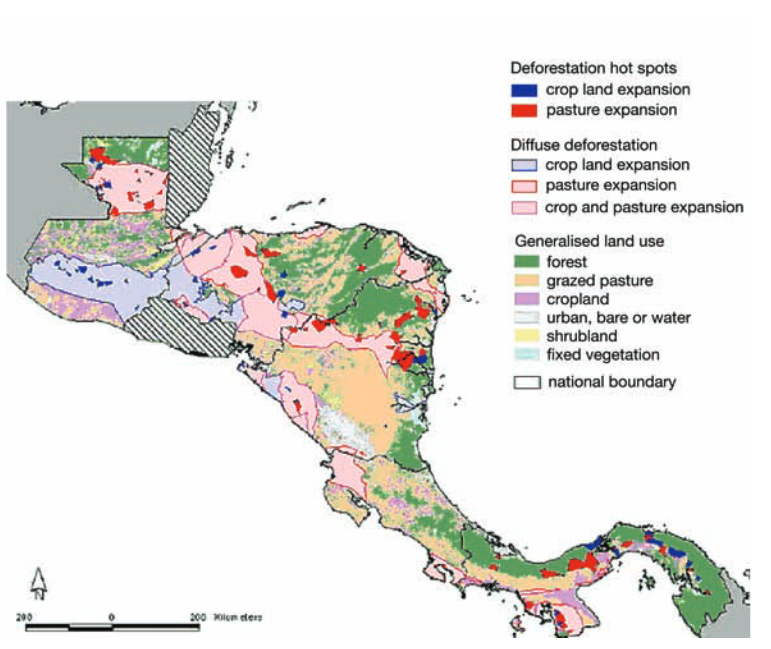
\includegraphics[width=0.75\textwidth]{lc_ca}
	\caption[Central America Land Usage]{Land usage and land cover change in Central America \citep{ipcc_2007}.}
	\label{fig:lc_ca}
\end{figure}

\subsection{Northern Brazil}

\begin{figure}[!ht]
	\centering
	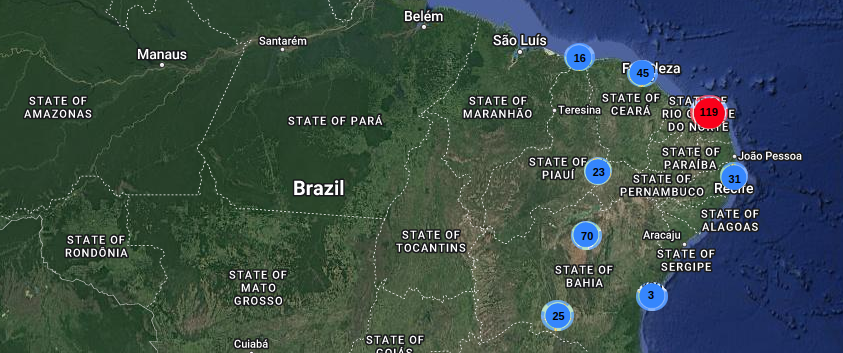
\includegraphics[width=0.75\textwidth]{maps_twp_sa}
	\caption[Northern Brazil Map]{Satellite image displaying Northern Brazil focus region from 65$^\circ$W to 30$^\circ$W longitude and 15$^\circ$S to 0$^\circ$S latitude \citep{maps_sa}. Markers indicating positions and number of wind farms have been edited on using data from \citep{twp_br}.}
	\label{fig:maps_twp_sa}
\end{figure}

\subsubsection{Description of region}

We selected the North to Northeast regions of Brazil (65$^\circ$W to 30$^\circ$W longitude and 15$^\circ$S to 0$^\circ$S latitude; see Figure~\ref{fig:maps_twp_sa}) because there has been extensive deforestation over this area and it was believed that effects resulting from \ac{LCC} here were likely to be especially pronounced. The change in \ac{MLAI} between these periods is displayed in Figure~\ref{fig:sa_lai_similar}.

\begin{figure}[!ht]
	\centering
	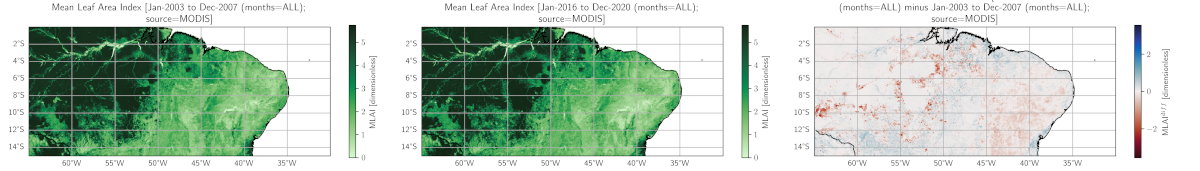
\includegraphics[width=0.9\textwidth]{sa_lai_similar.png}
	\caption[MLAI similar comparison for NB focus region]{\ac{MLAI} computed over each period in the similar comparison (left and middle), as well as the difference in these values between the two periods (right).}
	\label{fig:sa_lai_similar}
\end{figure}

\subsubsection{Significance of results from this region}

Several studies have identified large-scale changes in precipitation and moisture convergence patterns, which indirectly implicate surface wind changes. Effects here are likely to have immediate implications for energy generation due to the number of wind farms in this region (both existing and in the development pipeline\footnote{Up to 60 GW of offshore wind near the northeastern coast is in the early planning stage \citep{offshore_map}.}).

\subsubsection{Study periods}

For \ac{NB}, the selected periods for the similar comparison was from Jan-2002 to Dec-2006 and from Jan-2014 to Dec-2018 (for the same reasons highlighted in Section~\ref{sssec:period_seas_ca} for \ac{CA}.

\subsubsection{Land use and land cover change}

Figure~\ref{fig:lc_sa} displays trends in \ac{LULCC} at around the time of period 1 in the similar comparison.

\begin{figure}[!ht]
	\centering
	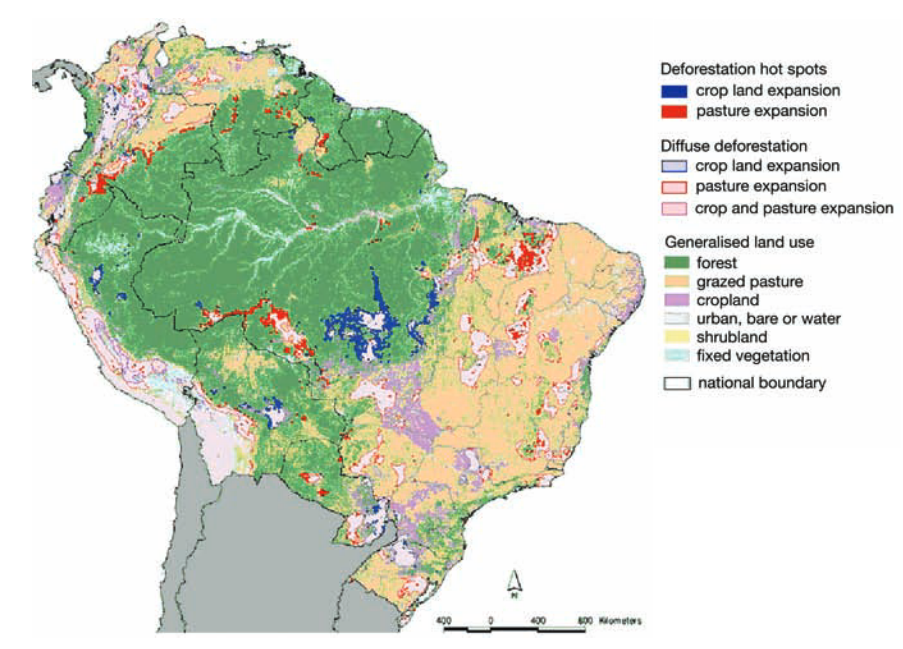
\includegraphics[width=0.75\textwidth]{lc_sa}
	\caption[Northern Brazil Land Usage]{Land usage and land cover change in Northern South America \citep{ipcc_2007}.}
	\label{fig:lc_sa}
\end{figure}     % these are just test names as I didn't know what you'd want
	\chapter{Data, files and codebooks}
\label{app:code}

\section{Availability and reproducible results}

\section{Description of analysis functions}

\blindtext[10]
    
	\chapter{Codebook and reproducibility}
\label{app:code}

All code created in the course of this project is available at \url{https://github.com/anthonylst6/thesis}. Programs created for automating analysis of an arbitrary \ac{ERA5} variable (in terms of mean diurnal profile statistics, hourly means and monthly means) were envisioned for general usage and as such, most of the functions within each script have been documented using Python docstrings, and permission to use these programs are granted subject to MIT License conditions.

\section{High-level description of functions}

\begin{itemize}
	\item The functions created in the course of this thesis allow comparison for the \acf{MLAI} and \acf{MFAPAR} between two arbitrary periods (so long as they are within the range of available data from 1981-2021). And the comparison can further be done in terms of a subset of months from each period. So it is possible, for example, to compare the \ac{MLAI} over the months of January, March and December between 1990-2000 with the \ac{MLAI} over the months of July and November between 2005-2007. These variables derive from the \ac{GLASS} dataset.
	\item These functions also allow comparison for various \ac{ERA5} variables between two arbitrary periods in terms of each variable's diurnal profile (can choose subset of months), mean (can choose subset of both months and hours), hourly means for each hour of the day (can choose subset of months), and monthly means for each month of the day (can choose subset of hours).
	\item For wind speed, there is also a separate function to compute the mean, standard deviation, Weibull distribution parameters resulting from an empirical fit, and other.
	\item The main data processing functions are contained in the \verb+calc_funcs.py+ script in the \verb+scripts+ folder.
	\item The \verb+plot_funcs.py+ script in the \verb+scripts+ folder is a plotting layer on top of \verb+calc_funcs.py+ and contains all the functions for creating comparison plots.
	\item Most analysis can be done purely using the \verb+plot_funcs.py+ script since this was built to automatically invoke any processing functions from \verb+calc_funcs.py+ if the processed data file does not already exist.
	\item The entire code is built around carefully selected names for each file, so it is not recommended to rename any of these files as this may break the code.
	\item There is a vast array of functions within these scripts but we will describe here only the high-level comparison plot functions. For detail into the other functions, look into the docstrings embedded within each script. At the time of writing, \verb+calc_funcs.py+ is fully documented while only the high-level comparison plot functions in \verb+plot_funcs.py+ have been documented.
	\item The high-level comparison plot functions in \verb+plot_funcs.py+ are: 
	\begin{itemize}
		\item \verb+plot_comp_mdp_clim_stats_given_var_or_dvar+
		\item \verb+plot_comp_means_given_layer_and_type+
		\item \verb+plot_comp_hourly_means_given_var_or_dvar+
		\item \verb+plot_comp_monthly_means_given_var_or_dvar+
		\item \verb+plot_comp_wsd_clim+
	\end{itemize}
	\item Each of these functions creates an output plot with 3 columns and 8 rows. The left column corresponds to the statistical summaries for the first period of study. The middle column is the same but for the second period. The right column is the difference between periods in the values for each statistical summary (calculated as second period minus first period). For reference, the first two rows will always display \ac{MLAI} and \ac{MFAPAR}. The colourbars are automatically standardised to allow fair comparison between periods, months and hours.
	\item Where spatiotemporal correlations in the left or middle columns hold between an \ac{ERA5} statistic and \ac{MLAI}, this is suggestive that the vegetation cover \textit{may} be responsible for the observed variations in the \ac{ERA5} statistic.
	\item Where spatiotemporal correlations hold between the right column of an \ac{ERA5} statistic and the left or middle columns for \ac{MLAI}, this leaves open the question of what is causing the observed variations in the \ac{ERA5} statistic, but suggests that vegetation cover \textit{may} be responsible for modulating these variations.
	\item Where spatiotemporal correlations hold between the right columns of an \ac{ERA5} statistic and \ac{MLAI}, this is suggestive that the variations in vegetation cover \textit{may} be responsible for the variations in the \ac{ERA5} statistic.
\end{itemize}

\section{Example usage}

\subsection{plot\_comp\_mdp\_clim\_stats\_given\_var\_or\_dvar}

Suppose we were interested in analysing the seasonal differences in the diurnal statistics of mean sea level pressure ("mslp") in a region of South America ("sa"), with default region extents manually defined in the \verb+calc_funcs.py+ script. Specifically, we are interested in differences between the wet season from January to June ([1,2,3,4,5,6]) and the dry season from July to December ([7,8,9,10,11,12]), over the period from "Jan-2001" to "Dec-2020". Then we would use the following code to obtain Figure~\ref{fig:plot_comp_mdp_clim_stats_given_var_or_dvar}:

\begin{lstlisting}[language=Python,caption={Example for plot\_comp\_mdp\_clim\_stats\_given\_var\_or\_dvar},captionpos=b]
	import plot_funcs_v1h as pf
	pf.plot_comp_mdp_clim_stats_given_var_or_dvar(
		region="sa", period1_start="Jan-2001", period1_end="Dec-2020", 
		period2_start="Jan-2001", period2_end="Dec-2020", 
		period1_months=[1,2,3,4,5,6], period2_months=[7,8,9,10,11,12], 
		glass_source_pref="modis", var_or_dvar="mslp", 
		perc=False, mask_perc_quantile=pf.mask_perc_quantile_default, 
		mask_period1=None, mask_period2=None, extents=None, cfv_data=None, 
		output=True
	)
\end{lstlisting}

\begin{figure}[!htp]
	\centering
	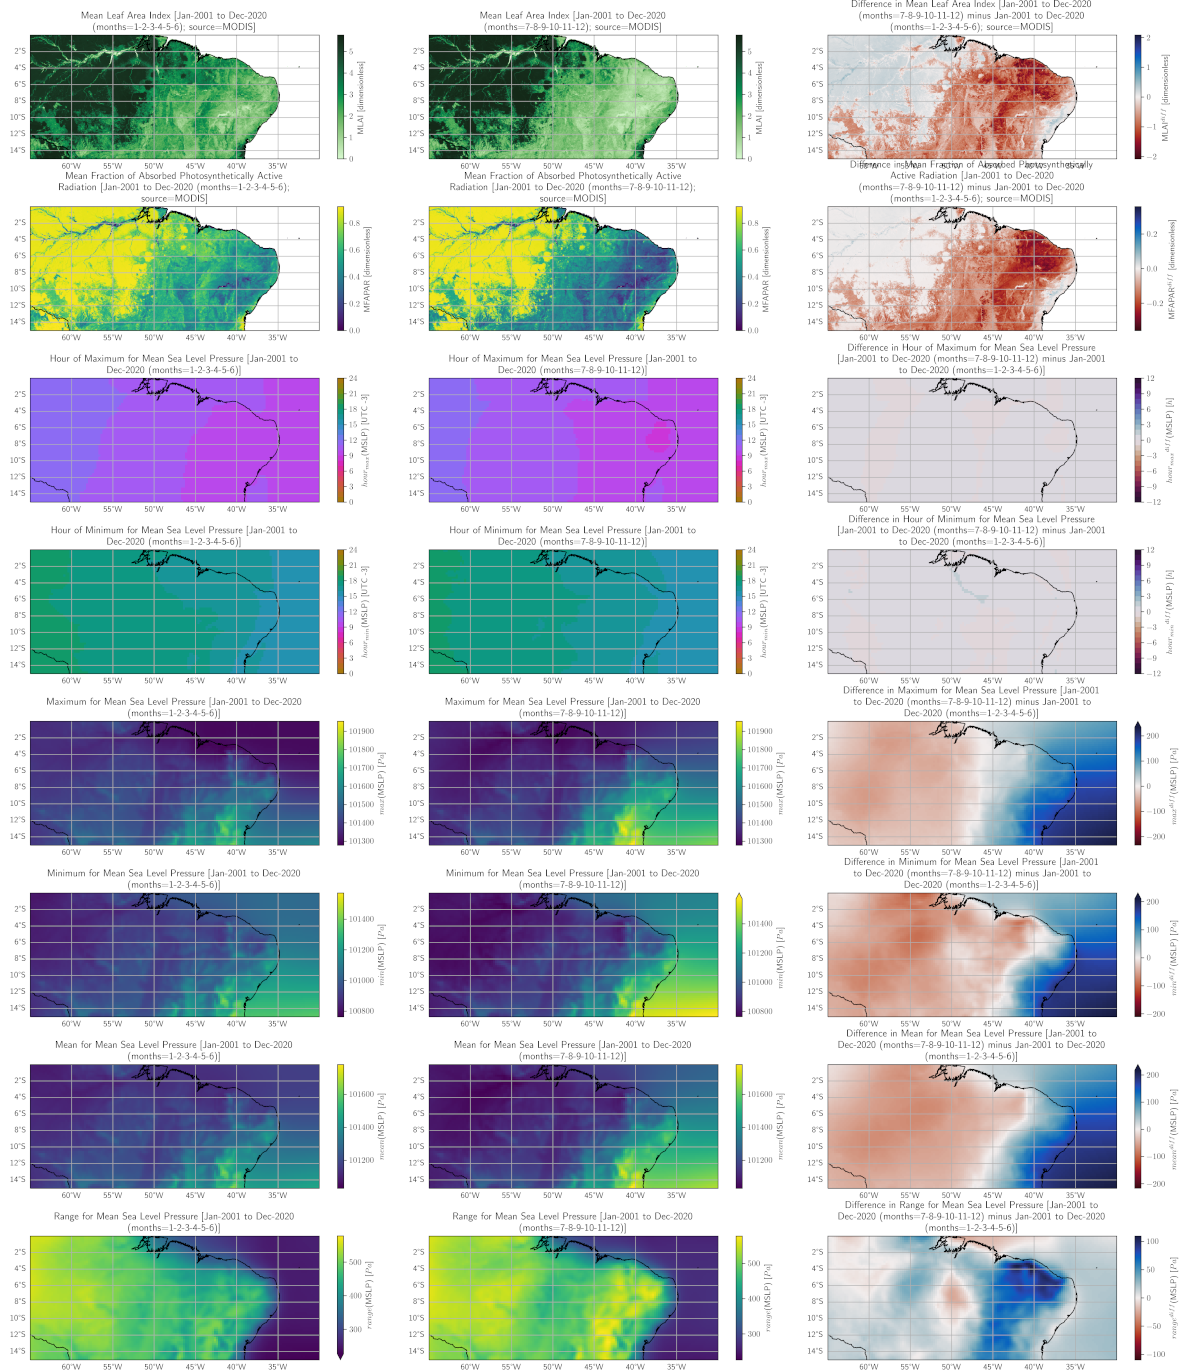
\includegraphics[width=0.9\textwidth]{plot_comp_mdp_clim_stats_given_var_or_dvar}
	\caption{Example for plot\_comp\_hourly\_means\_given\_var\_or\_dvar}
	\label{fig:plot_comp_mdp_clim_stats_given_var_or_dvar}
\end{figure}

\subsection{plot\_comp\_means\_given\_layer\_and\_type}

Suppose we were interested in analysing differences in the means between two separate periods for the hourly change in variables ("dvars") at the surface ("sfc"), in a region of Central America ("ca"), with default region extents manually defined in the \verb+calc_funcs.py+ script. Specifically, we are interested in differences in means computed over daytime hours from 0800 to 1500 ([8,9,10,11,12,13,14,15]) and the wet season from May to October ([5,6,7,8,9,10]), between the periods from "Jan-2003" to "Dec-2007" and "Jan-2016" to "Dec-2020". Then we would use the following code to obtain Figure~\ref{fig:plot_comp_means_given_layer_and_type}:

\begin{lstlisting}[language=Python,caption={Example for plot\_comp\_means\_given\_layer\_and\_type},captionpos=b]
	import plot_funcs_v1h as pf
	pf.plot_comp_means_given_layer_and_type(
		region="ca", period1_start="Jan-2003", period1_end="Dec-2007", 
		period2_start="Jan-2016", period2_end="Dec-2020", 
		period1_months=[5,6,7,8,9,10], period2_months=[5,6,7,8,9,10], 
		period1_hours=[8,9,10,11,12,13,14,15], 
		period2_hours=[8,9,10,11,12,13,14,15], 
		glass_source_pref="modis", 
		var_or_dvar_layer="sfc", var_or_dvar_type="dvars", 
		perc=False, mask_perc_quantile=pf.mask_perc_quantile_default, 
		mask_period1=None, mask_period2=None, extents=None, cfv_data=None, 
		output=True
	)
\end{lstlisting}

\begin{figure}[!htp]
	\centering
    \begin{subfigure}[!htp]{0.9\textwidth}
		\centering
		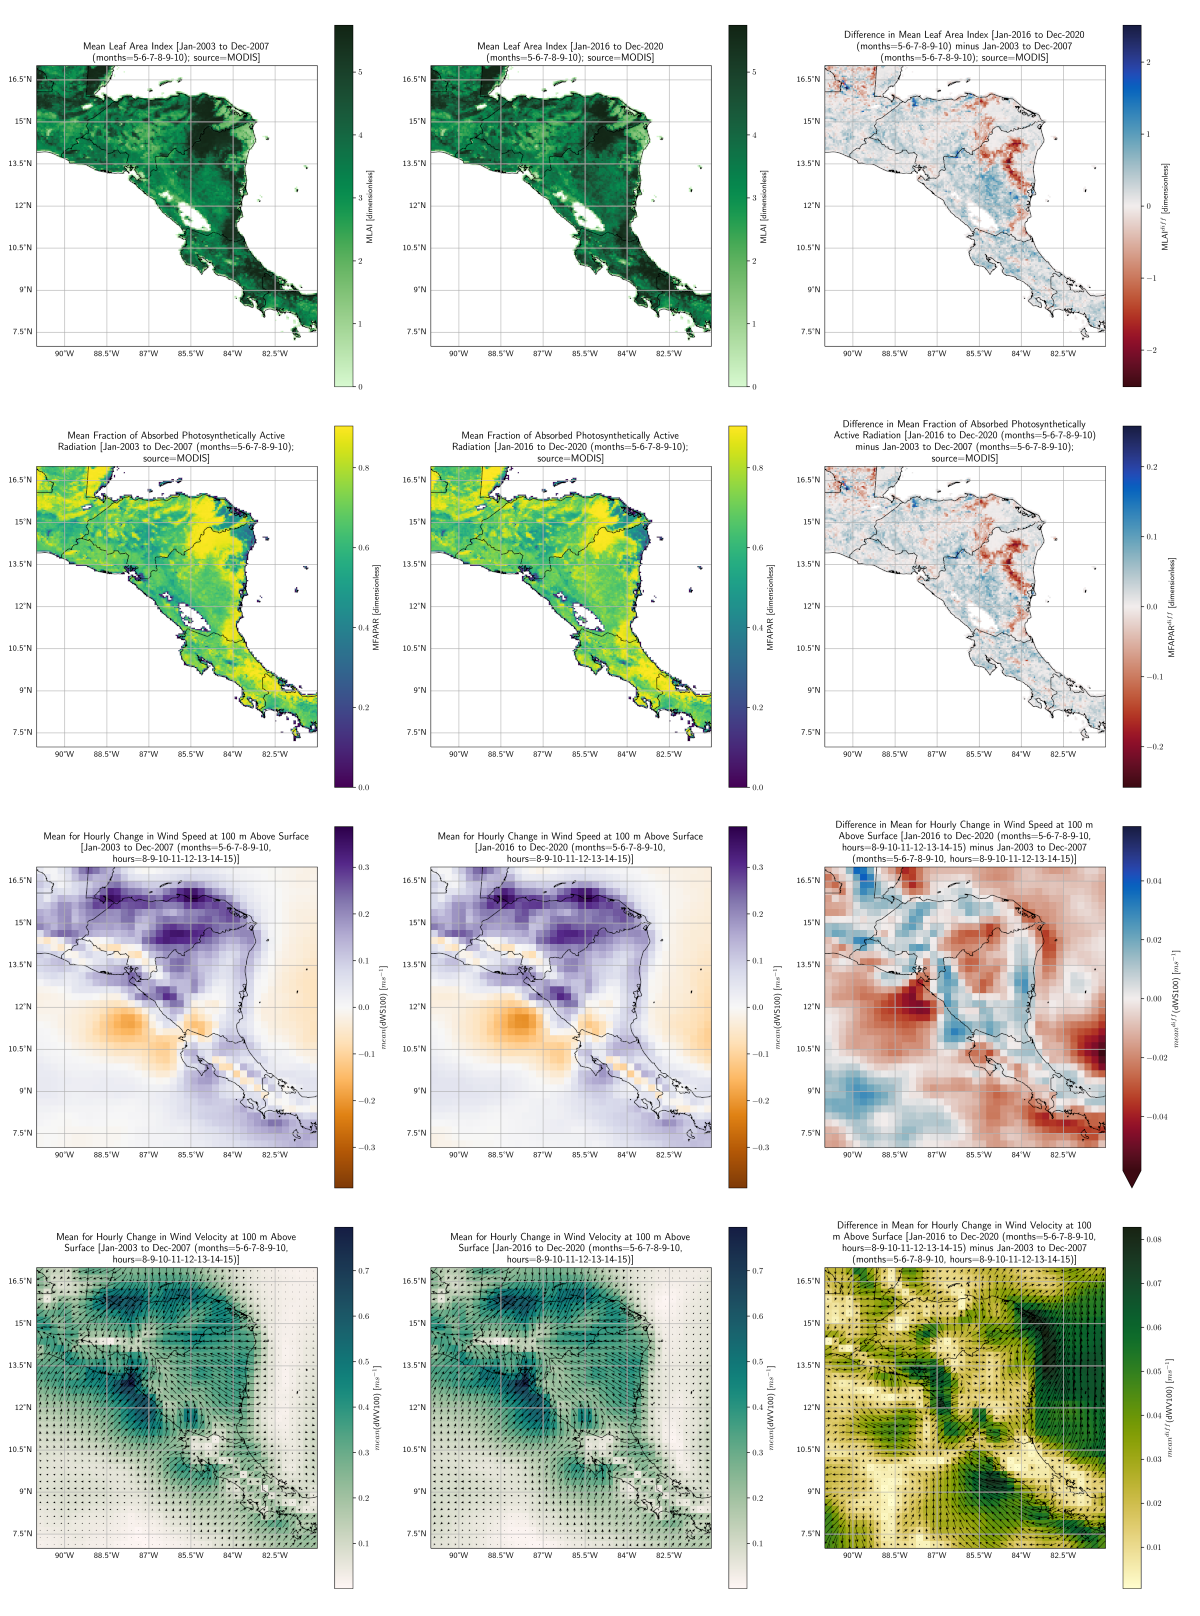
\includegraphics[width=0.9\textwidth]{plot_comp_means_given_layer_and_type_1}
		\caption[]{First 4 rows of example plot}
	\end{subfigure}
\end{figure}

\begin{figure}[!htp]\ContinuedFloat
    \begin{subfigure}[!htp]{0.9\textwidth}
		\centering
		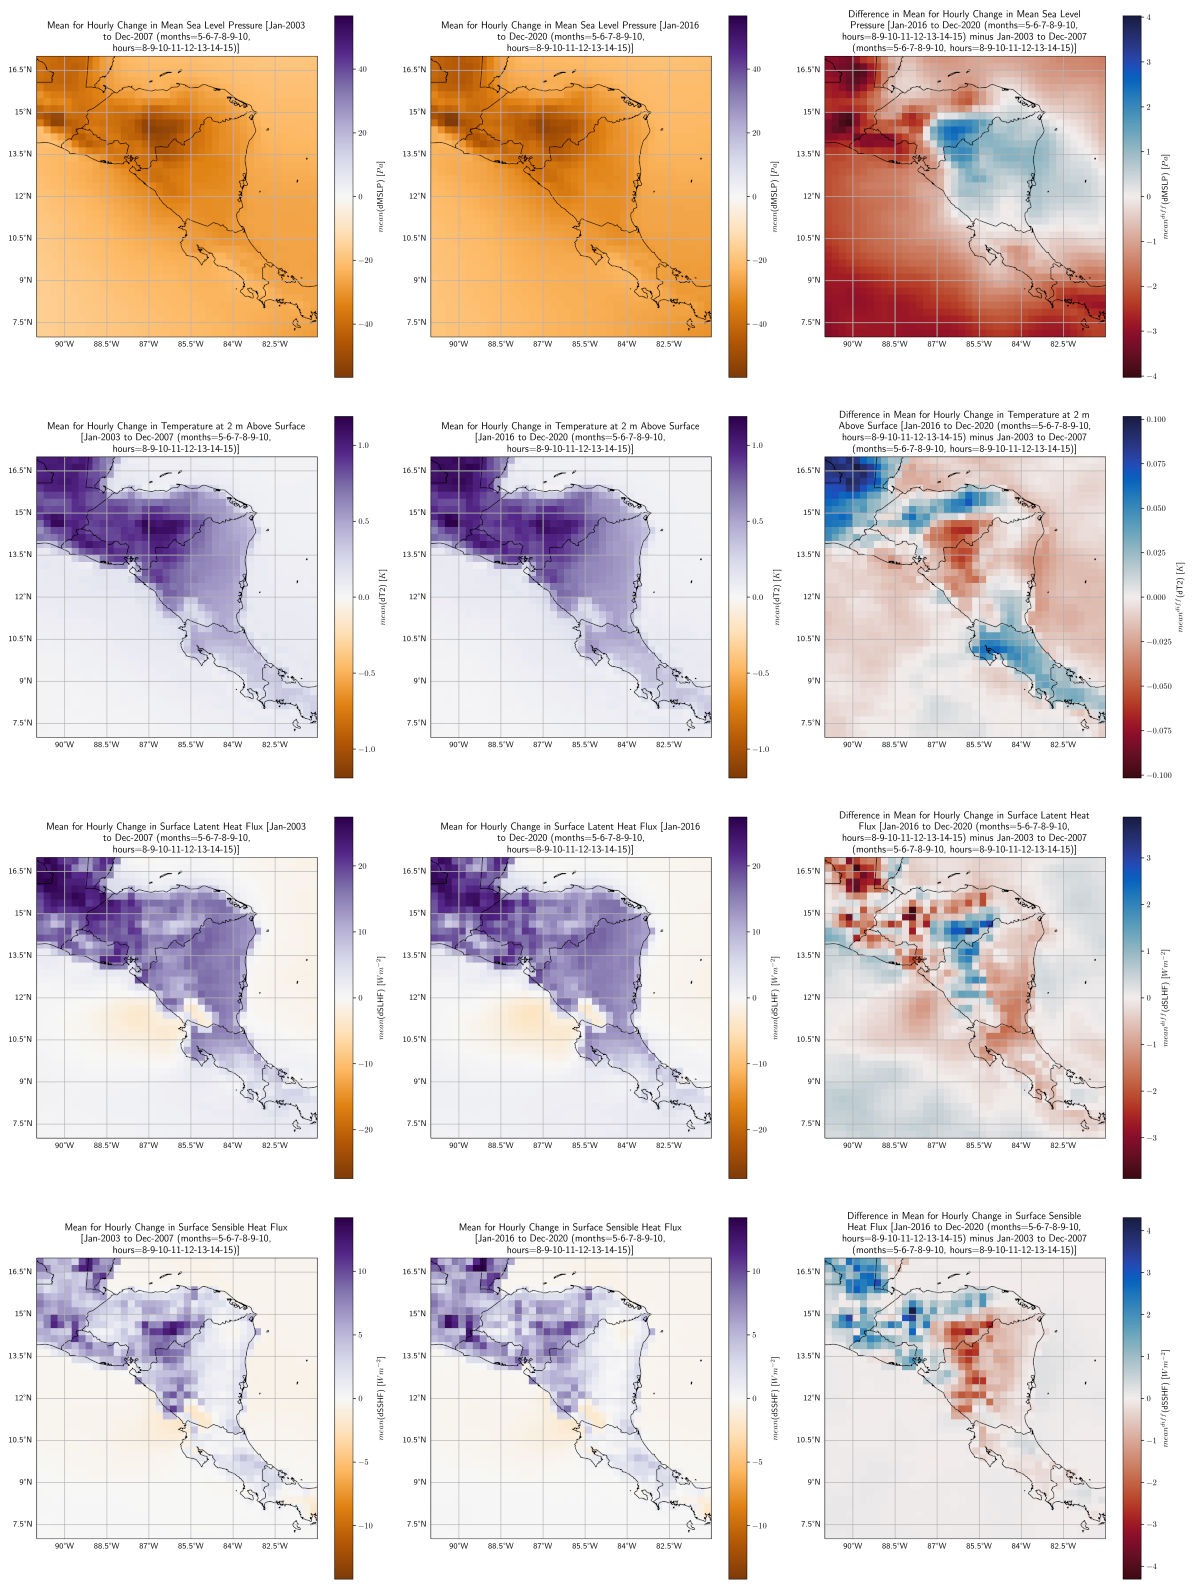
\includegraphics[width=0.9\textwidth]{plot_comp_means_given_layer_and_type_2}
		\caption[]{Last 4 rows of example plot}
	\end{subfigure}
	\caption{Example for plot\_comp\_means\_given\_layer\_and\_type}
	\label{fig:plot_comp_means_given_layer_and_type}
\end{figure}

\subsection{plot\_comp\_hourly\_means\_given\_var\_or\_dvar}

Suppose we were interested in analysing the seasonal differences in the hourly means of vertical integral of energy conversion ("viec") in a region of Western Australia ("wa"), with default region extents manually defined in the \verb+calc_funcs.py+ script (and the State Boundary Fence of Western Australia is drawn in). Specifically, we are interested in differences between the wet season from July to August ("jja") and the dry season from December to February ("djf"), over the period from "Jan-2001" to "Dec-2020". Then we would use the following code to obtain Figure~\ref{fig:plot_comp_hourly_means_given_var_or_dvar}:

\begin{lstlisting}[language=Python,caption={Example for plot\_comp\_hourly\_means\_given\_var\_or\_dvar},captionpos=b]
	import plot_funcs_v1h as pf
	pf.plot_comp_hourly_means_given_var_or_dvar(
		region="wa", period1_start="Jan-2001", period1_end="Dec-2020", 
		period2_start="Jan-2001", period2_end="Dec-2020", 
		period1_months="jja", period2_months="djf", glass_source_pref="modis", 
		var_or_dvar="viec", hours_to_plot="18-23", 
		perc=False, mask_perc_quantile=pf.mask_perc_quantile_default, 
		mask_period1=None, mask_period2=None, extents=None, cfv_data=None, 
		output=True
	)
\end{lstlisting}

\begin{figure}[!htp]
	\centering
	\begin{subfigure}[!htp]{0.9\textwidth}
		\centering
		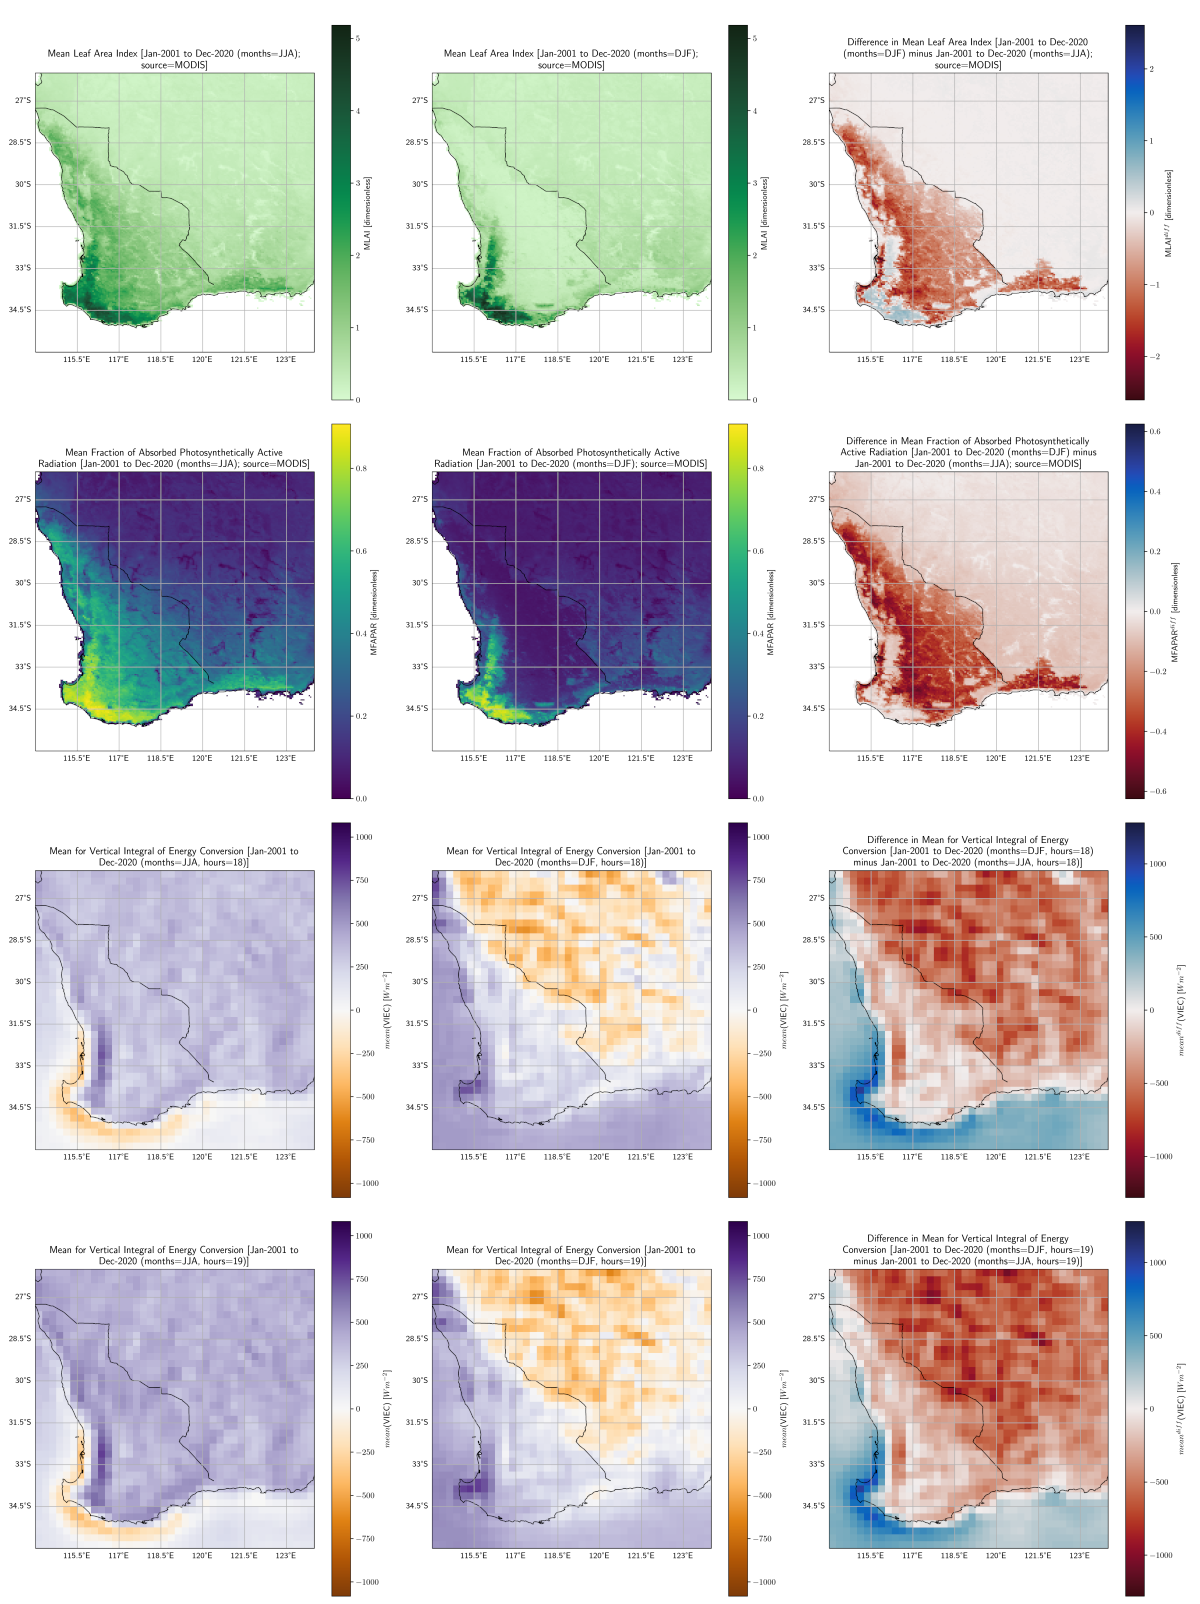
\includegraphics[width=0.9\textwidth]{plot_comp_hourly_means_given_var_or_dvar_1}
		\caption[]{First 4 rows of example plot}
	\end{subfigure}
\end{figure}

\begin{figure}[!htp]\ContinuedFloat
	\begin{subfigure}[!htp]{0.9\textwidth}
		\centering
		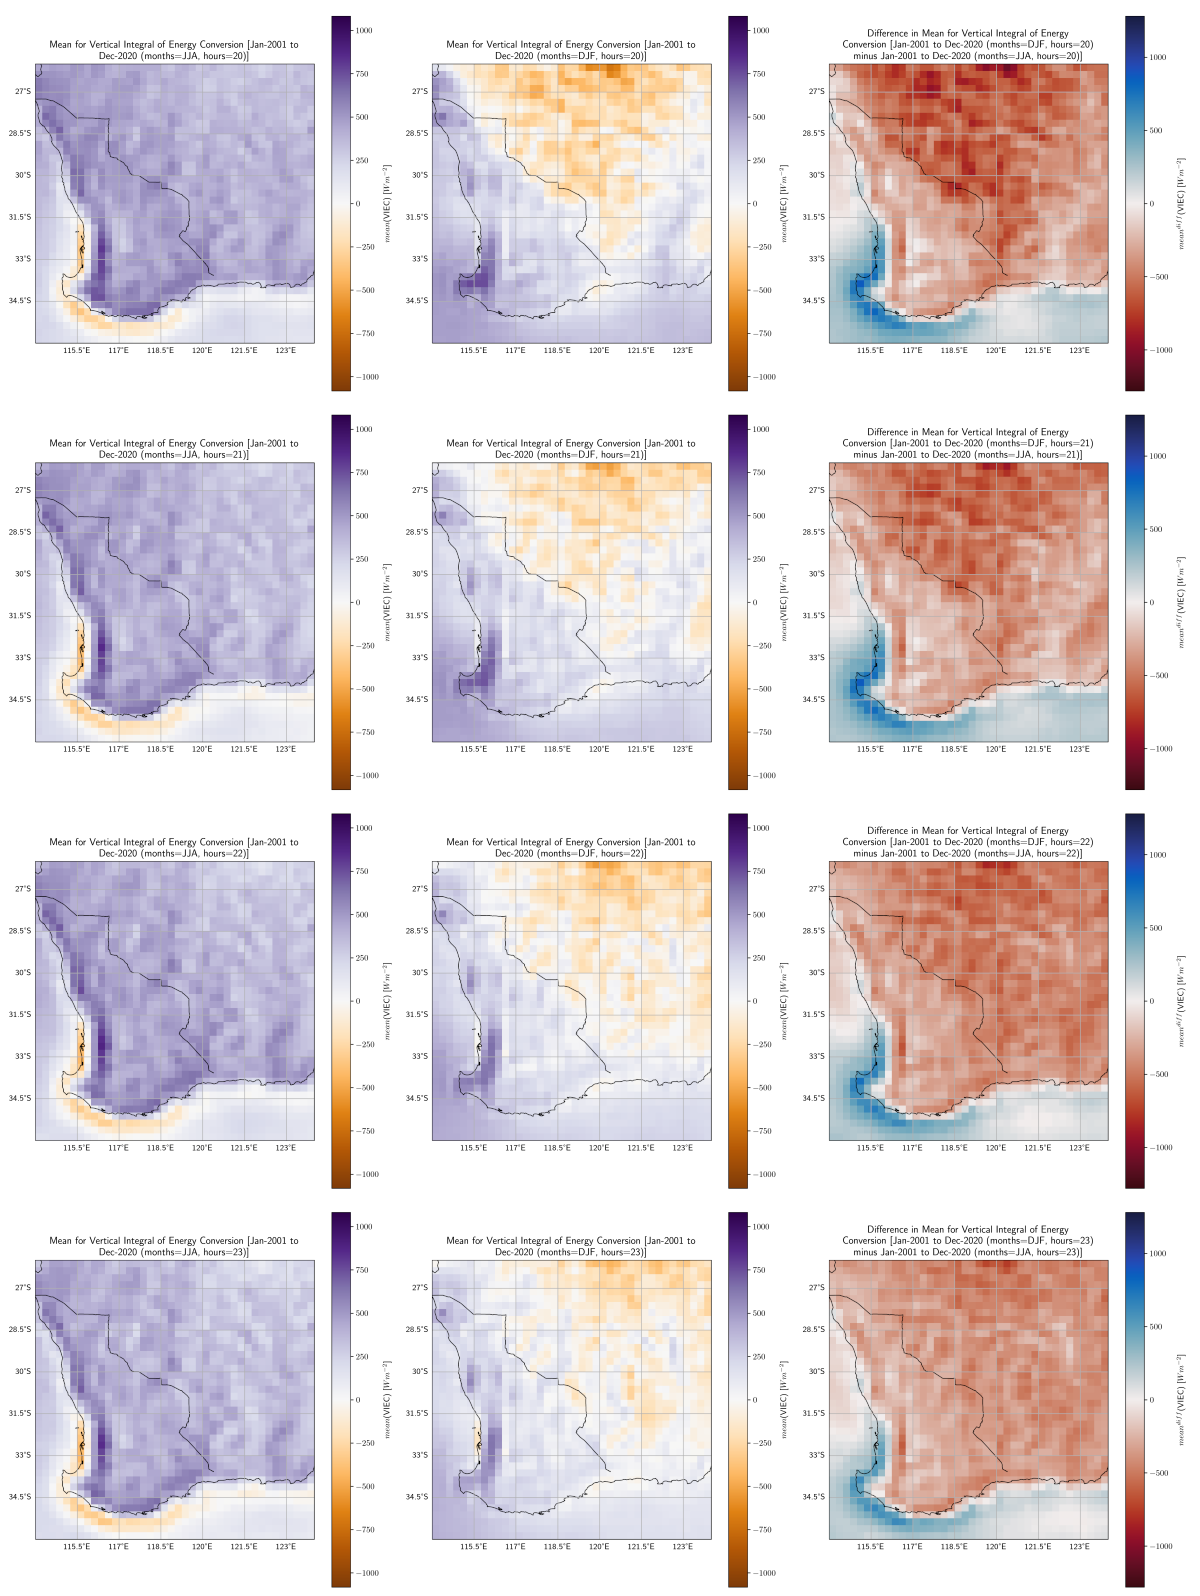
\includegraphics[width=0.9\textwidth]{plot_comp_hourly_means_given_var_or_dvar_2}
		\caption[]{Last 4 rows of example plot}
	\end{subfigure}
	\caption{Example for plot\_comp\_hourly\_means\_given\_var\_or\_dvar}
	\label{fig:plot_comp_hourly_means_given_var_or_dvar}
\end{figure}

\section{Analysing other regions and variables}

Note: the steps in this section have not been tested as of the time of writing.

\subsection{For custom regions}

\begin{itemize}
	\item The default regions and extents in [W, E, S, N] format (for \verb+cartopy+ plotting library) used in the thesis project were: 
	\begin{itemize}
		\item "wa": [114, 124, -36, -26]
		\item "ca": [-91, -81, 7, 17]
		\item "sa": [-65, -30, -15, 0]
	\end{itemize}
	\item To add a custom region:
	\begin{enumerate}
		\item Edit the \verb+area+ variable in \verb+data_download.ipynb+ or \verb+data_download.py+ to include the name of the new region and its extents in [N, W, S, E] format (for \ac{ECMWF} \ac{CDS} API)
		\item Edit the first argument in the \verb+retrieve_era5_slv_month_hour+ and \\ \verb+retrieve_era5_slv_hour+ functions so that it reflects the name of the new region
		\item Run the edited \verb+data_download.ipynb+ or \verb+data_download.py+ to download the relevant \ac{ERA5} data from \ac{ECMWF}
		\item Edit the \verb+regions+ variable in the \verb+calc_funcs.py+ script to include the new region's name, extents in [W, E, S, N] format, and local timezone relative to UTC
	\end{enumerate}
\end{itemize}

\subsection{For arbitrary ERA5 variables}

\begin{itemize}
	\item The ERA5 variables obtained from \ac{ECMWF} for use in the thesis project by default were (using naming conventions from \url{https://confluence.ecmwf.int/display/CKB/ERA5%3A+data+documentation}):
		\begin{itemize}
			\item \verb+'100m_u_component_of_wind'+
			\item \verb+'100m_v_component_of_wind'+
			\item \verb+'10m_u_component_of_wind'+
			\item \verb+'10m_v_component_of_wind'+
			\item \verb+'2m_temperature'+
			\item \verb+'mean_sea_level_pressure'+
			\item \verb+'surface_latent_heat_flux'+
			\item \verb+'surface_sensible_heat_flux'+
			\item \verb+'evaporation'+
			\item \verb+'total_column_cloud_liquid_water'+
			\item \verb+'total_column_water_vapour'+
			\item \verb+'vertical_integral_of_divergence_of_moisture_flux'+
			\item \verb+'vertical_integral_of_energy_conversion'+
			\item \verb+'vertical_integral_of_kinetic_energy'+
			\item \verb+'convective_inhibition'+
			\item \verb+'forecast_albedo'+
			\item \verb+'total_cloud_cover'+
		\end{itemize}
	\item To add an arbitrary \ac{ERA5} variable:
	\begin{enumerate}
		\item Edit the \verb+vars_era5+ variable in \verb+data_download.ipynb+ or \\ \verb+data_download.py+ to include the name of the new variable using the \ac{ERA5} variable names from \url{https://confluence.ecmwf.int/display/CKB/ERA5%3A+data+documentation}
		\item Place the variable within one of the existing "sfc", "atm" or "cld" categories
		\item (Alternatively) Create a new category with the variable and add additional code cells with the new category name as an argument into the \\ \verb+retrieve_era5_slv_month_hour+ and \\ \verb+retrieve_era5_slv_hour functions+
		\item Run the edited \verb+data_download.ipynb+ or \verb+data_download.py+ to download the relevant \ac{ERA5} data from \ac{ECMWF} \ac{CDS}
		\item Edit the \verb+vars_and_dvars_era5+, \verb+vars_dep_and_rename+ and \verb+attrs_da+ variables in the \verb+calc_funcs.py+ script to reflect this new variable
		\item Edit the try-except blocks in the \verb+plot_means_given_layer_and_type+, \verb+plot_diff_means_given_layer_and_type+ and \\ \verb+plot_comp_means_given_layer_and_type+ functions in the \\ \verb+plot_funcs.py+ script so that a total of 6 \ac{ERA5} variables will be displayed at all times (this is an unfortunate design constraint from displaying 8 rows for the comparison plots with the first 2 rows occupied by \ac{MLAI} and \ac{MFAPAR})
	\end{enumerate}
\end{itemize}

\subsection{For novel ERA5-derived variables}

\begin{itemize}
	\item The default \ac{ERA5}-derived variables used in the thesis project were: 
	\begin{itemize}
		\item Instantaneous approximation (with negative sign reversed and units converted) for \acf{SLHF}
		\item Instantaneous approximation (with negative sign reversed and units converted) for \acf{SSHF}
		\item Instantaneous approximation (with negative sign reversed and units converted) for \acf{NSE}
		\item Approximation for \acf{NAC}
	\end{itemize}
	\item To incorporate a novel \ac{ERA5}-derived variable:
	\begin{enumerate}
		\item Insert an if statement into the \verb+calc_era5_mdp_clim_given_var_or_dvar+ function in the \verb+calc_funcs.py+ script (this is the function which is furthest upstream and from which other computations apart from wind speed distribution derive from) using the same style and logic as that for \ac{NAC} in the script
		\item Edit the \verb+vars_and_dvars_era5+, \verb+vars_dep_and_rename+ and \verb+attrs_da+ variables in the \verb+calc_funcs.py+ script to reflect this new variable
		\item Edit the try-except blocks in the \verb+plot_means_given_layer_and_type+, \verb+plot_diff_means_given_layer_and_type+ and \\ \verb+plot_comp_means_given_layer_and_type+ functions in the \\ \verb+plot_funcs.py+ script so that a total of 6 ERA5 variables will be displayed at all times (this is an unfortunate design constraint from displaying 8 rows for the comparison plots with the first 2 rows occupied by \ac{MLAI} and \ac{MFAPAR})
	\end{enumerate}
\end{itemize}

\section[Steps to reproduce thesis]{Steps to reproduce thesis results from scratch}

Note: The original project scope included analysis for \ac{WA}, \ac{CA} and \ac{NB} but this was cut short to only \ac{WA} due to time constraints.

\begin{enumerate}
	\item (If haven't already) Install miniconda for Python 3.9 or later using instructions from \url{https://docs.conda.io/en/latest/miniconda.html}
	\item Download thesis repository by entering \\ \verb+git clone git@github.com:anthonylst6/thesis.git+ into a bash shell (Terminal for Linux or Mac, Git Bash recommended for Windows) or clicking Code -> Download ZIP on Github then unzip the folder
	\item Open bash shell in home directory of repository then run \\ \verb+conda env create -f env_thesis.yml+
	\item (If haven't already) Set up \ac{ECMWF} \ac{CDS} API using instructions from \url{https://confluence.ecmwf.int/display/CKB/How+to+download+ERA5#HowtodownloadERA5-4-DownloadERA5familydatathroughtheCDSAPI}
	\item Download raw data by entering \verb+conda activate thesis+ into bash shell then running the \verb+data_download.ipynb+ notebook in the \verb+scripts+ directory (open the notebook by running \verb+jupyter lab &+ in the bash shell)
	\item (Alternatively) Enter \verb+conda run -n thesis python data_download.py+ \\ into bash shell from the \verb+scripts+ directory
	\item (For proper rendering of figures) Make sure that a \LaTeX distribution is installed
	\item Reproduce results by running the \verb+results.ipynb+ notebook in the \verb+scripts+ directory for different focus regions by commenting and uncommenting relevant code (again use \verb+jupyter lab &+ from bash shell to open notebooks)
	\item (Alternatively) Enter \verb+conda run -n thesis python results_wa.py+, \\ \verb+conda run -n thesis python results_ca.py+ and \\ \verb+conda run -n thesis python results_sa.py+ into bash shell from the \\ \verb+scripts+ directory
	\item (If personal computer is limited in RAM) Edit the \verb+results_wa.pbs+, \\ \verb+results_ca.pbs+ and \verb+results_sa.pbs+ job scripts in the \verb+scripts+ directory to be compatible with target HPC facility (the provided scripts were designed for the UNSW Katana computational cluster), then submit these as a batch job
\end{enumerate}

\section[System and time requirements]{System and time requirements (for reproducing thesis results only)}
\begin{itemize}
	\item For \acf{WA} raw data and results, up to 25 GB of storage, several days for raw data download (due to queueing in \ac{ECMWF} \ac{CDS}), and for data processing up to 60 GB of RAM over 12 hours if using 8 CPUs
	\item For \acf{CA} raw data and results, up to 25 GB of storage, several days for raw data download (due to queueing in \ac{ECMWF} \ac{CDS}), and for data processing up to 60 GB of RAM over 12 hours if using 8 CPUs
	\item For \acf{NB} raw data and results, up to 80 GB of storage, several days for raw data download (due to queueing in \ac{ECMWF} \ac{CDS}), and for data processing up to 140 GB of RAM over 12 hours if using 8 CPUs
	\item The data processing can also be run with less RAM and fewer CPU cores but this will be slower and will require manual restarting of code everytime RAM limit is reached (the code was designed to pick up from where it left off). But in this case there should at least be 8 GB of RAM for \ac{WA} and \ac{CA} results, and at least 24 GB of RAM for \ac{NB} results.
\end{itemize}
 




\end{document}

%%% The End %%%
